\section{Control system architecture}
\label{sec:Chap3-ControlSystemArchitecture}
Chapter~\ref{chap:phasenoisepaper} sets the general background to double-Fourier interferometry when used mostly in spectroscopy mode. It sets the mathematical formalism to estimate the spectral sensitivity, given various sources of gaussian noises. 

In this section, we see more directly how this applies to BETTII, and how the system is designed to satisfy these requirements in order to guarantee good observations.

\subsection{Overall strategy}

\subsubsection{Requirements}
The strategy that we developed aims at satisfying the requirements established in the previous section, under the cost, time and personnel constraints that we were subject to. It fundamentally relies on the fact that \textit{knowledge} is more important than \textit{control}. While several research groups [CITE WASPS] are attempting to provide sub-arcsecond balloon gondola control, we are not going to. This strategy uses the fundamental advantage that the interferometer has over traditional pointed observatories: the decoupling of the phase with the pointing. This feature of interferometers refers to the possibility of obtaining electromagnetic interference even when the telescopes are slightly mispointed from the target. 

There three levels of requirements for our instrument to produce interferograms. First, both arms need to be pointed at the target, so that an image of the target seen through each arm is formed at the detector. For our purpose this will largely be set by the limitation of the field of view of the instrument, which is about 2 arcminutes. When a target is not exactly on-axis with the telescope, it can still fall on the detector if tip/tilt correction happens downstream. The tip/tilt correction will create aberrations, but these are relatively well behaved at our wavelengths. Hence, this requirement can be expressed as an overall pointing requirement of the instrument to some amount that can be corrected in tip/tilt in each individual arms. We set this to $\pm\ang{;;15}$. This also roughly corresponds to one single pixel on the short band detector, and half a primary beam's FWHM.

Once the instrument is pointed to the desired target to within $\pm\ang{;;15}$, there needs to be a fine guiding system in each arm that allows for the remaining correction. This level of control needs to overlap the beams to a small fraction of a pixel to get maximum overlap and minimum visibility losses. We set this requirement to \ang{;;1.5} r.m.s., which corresponds to a tenth of a pixel's size. The fine guidance system needs to operate over a range of at least $\pm\ang{;;15}$ to pick up where the previous level of requirements stops. It also needs to happen with high bandwidth to ensure that only minimum motion is occurring at timescales comparable to a data acquisition timescale. This system is described in section [].

Finally, an angular mispointing of the baseline vector with respect to the target can be might still exist, even if both beams are overlapped properly. This introduces an unwanted optical delay that can push the fringe packets outside our nominal OPD scanning range. Control of this optical delay is critical for interferometry, as it is required to properly reconstruct the OPD axis of the interferograms that are the elementary data blocks of the instrument. This can be achieved using a delay line . This is commonly done for all interferometers on the ground [CITE], and we will implement a device like this on BETTII as well [section]. For this to work, we need to be able to monitor the changes in OPD accurately, which is equivalent, on short timescales, to accurately estimate the attitude of the payload.


%\begin{figure}[!ht]
%	\centering
%	\includestandalone{Figures/InterferometryBaseline}
%	\caption[Relationship between pointing error and OPD]{Relationship between pointing error and OPD}
%	\label{fig:interferometrybaseline}
%    \end{figure}
%

A good estimate of the attitude of our payload can lead to an accurate angular difference between our baseline vector and our target. This angular difference can be converted to an OPD using simple geometric arguments, and can then be fed to the delay line for correction. With an 8~m baseline length, an mispointing of \ang{;;1} along the baseline direction corresponds to an OPD of about \SI{40}{\um}, or one full wavelength of BETTII's short-wavelength band. In order to produce quality interferograms, we will need to know the OPD to a fraction of this [SEE previous section]. 



\subsubsection{Control loop design and operating modes}

The three levels of control that we need are:
\begin{enumerate}
\item Coarse control of the entire gondola to within $\pm~$\ang{;;15} of the target,
\item Fine pointing control of each beam to \ang{;;1.5} r.m.s. at the science detector,
\item Fine knowledge of the inertial attitude to $\approx$~\ang{;;0.15} r.m.s., followed by appropriate OPD control
\end{enumerate}

At its fundamental level, the problem is to implement a system that satisfies these requirements, starting with only the target's location in right ascension (RA) and declination (DEC). Ideally, the system needs to be able to achieve these goals autonomously. All of the operating modes follow from this.

All of the pointing will be done in the reference frame of the gondola, which is tied solidly to the reference frame of the gondola (nominally they are the same) and the star cameras (nominally off by \SI{-45}{\degree} about the $\vectors{y}$~axis. In the following sections, we describe how the inertial attitude of the gondola is determined. Once it is known, a target's RA and DEC can be converted to a desired local azimuth $\Az$ and elevation $\El$ in the spherical coordinates attached to the gondola reference frame (see Fig.~\ref{fig:AzEl}). It is important to note that when we mention "azimuth", we are not referencing to any cardinal directions, as it can be done for other applications. For us, an azimuth is one of the two spherical angles that describe the position of our target in the current gondola reference frame. Note that the elevation angle is defined as being zero in the ($\vectors{x}_\gyro$,$\vectors{y}_\gyro$)-plane.

\begin{figure}[!ht]
	\centering
	\includestandalone{Figures/AzEl}
	\caption[Azimuth and elevation of a target]{}
	\label{fig:AzEl}
    \end{figure}


Once the turbulence from the ascent have died out, the control system determines where the gondola is currently pointing using the star cameras. For the software to process the star camera image, the payload has to be still to avoid blurring of the stars on the CCD. Hence, the first order of business is to slow down the payload's inertial velocity, which is measured by the gyroscopes. This is also called $\BRAKE$ mode.

The first time the system receives a star camera frame and identifies its inertial position, this triggers the estimator algorithm that constantly combines gyroscope and star camera information. From this point on, we have a reasonable estimate of where the gyroscope reference frame is pointed in the inertial frame at all times. 

When a new target in RA and DEC is set by the flight computer, the system will enter the $\SLEW$ mode. This creates a profile of desired azimuth position and velocity as a function of time. The software actuates the reaction wheels to turn the payload about its $\vectors{z}$ axis. At the same time, it commands the rotation stages that control the telescopes' elevation, to go to the desired elevation. The control in elevation and control in azimuth are entirely decoupled.

When we complete the deceleration phase as we get close to our target, we switch to $\TRACK$ mode. This mode is attempting at maintaining control of the telescope within $\pm$~\ang{;;15} of our target.

Finally, for each of the two arms, we need to acquire a guide star onto our guide camera [section]. This requires a fast imaging capability and a fast-steering tip/tilt correction mechanism to freeze the motion of the sky on the guide camera. This is $\ACQUIRE$ mode. Two images of the sky are made on the detector, one from each arm; the guide star is located in each image, and the tip/tilt mechanisms are actuated to center this star onto a location of the detector that corresponds to maximum overlap at the science detectors. One the star is centered onto that location, the window size of the camera decreases, and the acquisition speed increases. Ultimately, we will get two patches of 35$\times$35 pixels at $\approx$~\SI{50}{\hertz}. When this acquisition speed is reached we consider ourselves in $\LOCKED$ mode.

In both $\ACQUIRE$ and $\LOCKED$ mode, the position of the two tip/tilt platforms contains information on the overall mispointing of the optical train: when the actuators are both off in the same direction with respect to their nominal position, it means that the entire truss is off the guide star by this amount. When available, this information is used by the estimator along with the gyroscope and star camera information to compute the best possible attitude estimate. Since the tip/tilt is tied to the actual optics train, its information is heavily weighted compared to the other sensors. 

When the two guide star images are centered, this means proper overlap of the far-infrared beams at the science detectors. Hence, we are in a position to spot interferometric signal, which will translate to a modulation of the intensity of the coherently combined image as a function of OPD. The OPD is constantly modulated with the Cold Delay Line [section], independently of the mode in which we are. However, residual mispointings can create large unwanted OPD perturbations. Hence, during $\TRACK$ and $\ACQUIRE$ mode, the Warm Delay Line mechanism is activated. Its goal is to use the estimated change in baseline position to predict the resulting OPD variations - and correct them directly in OPD space. 

During the $\LOCKED$ mode, we need to consider what happens if we lose the guide star. Since the field of view is relatively small compared to the expected motions of the gondola, the guide star could technically walk outside the range of the guide camera - at which point the attitude estimation relies temporarily on the gyroscopes as we switch back to $\ACQUIRE$ mode and the guide camera increases its field of view (and decreases its speed) until it finds the guide star.

\renewcommand{\arraystretch}{1.5}
\newlength\mylen
\settowidth\mylen{\textbullet}
\addtolength\mylen{-3mm}
\setlist[itemize,1]{nolistsep,leftmargin=*,labelsep=-\mylen}
\def\labelitemi{--}
\begin{table}[htbp]
\small
\begin{longtable}{cp{5cm}p{2.5cm}p{3.5cm}}
\toprule
Mode  & Description &  Actuators & Sensors \\
\midrule
$\SAFE$ & All PID gains set to 0; siderostats point towards zenith; azimuth is not commanded;  used during ascent, emergencies &
\begin{minipage}[t]{\linewidth}%
\begin{itemize}[align=parleft]
\item CDL
\end{itemize}
\end{minipage} &
\begin{minipage}[t]{\linewidth}%
\begin{itemize}[align=parleft]
\item Gyros
\item Star cameras
\end{itemize}
\end{minipage} \\
\hline
$\BRAKE$ & Used to slow down the payload after undesired motion; derivative gains only, no position loop & 
\begin{minipage}[t]{\linewidth}%
\begin{itemize}[align=parleft]
\item CCMG 
\item Rotators
\item  CDL
\item  Mom. Dump
\end{itemize}
\end{minipage} &
\begin{minipage}[t]{\linewidth}%
\begin{itemize}[align=parleft]
\item Gyros
\item Star cameras 
\item Elevation encoder 
\item Gimbal encoder
\end{itemize}
\end{minipage} \\
\hline
$\SLEW$ &Used to move to target with a set velocity profile &
\begin{minipage}[t]{\linewidth}%
\begin{itemize}[align=parleft]
\item CCMG 
\item  Rotators
\item  CDL
\item  Mom. Dump
\end{itemize}
\end{minipage} &
\begin{minipage}[t]{\linewidth}%
\begin{itemize}[align=parleft]
\item Gyros 
\item Star cameras  
\item Elevation encoder  
\item Gimbal encoder
\end{itemize}
\end{minipage}\\
\hline
$\TRACK$ & Used to stabilize payload after slew, track target coarsely &
\begin{minipage}[t]{\linewidth}%
\begin{itemize}[align=parleft]
\item CCMG 
\item  Rotators
\item  CDL
\item  Mom. Dump
\item  WDL
\end{itemize}
\end{minipage} &
\begin{minipage}[t]{\linewidth}%
\begin{itemize}[align=parleft]
\item Gyros
\item  Star cameras 
\item  Elevation encoder 
\item  Gimbal encoder
\end{itemize}
\end{minipage}\\
\hline
$\ACQUIRE$ & The guide camera grabs images for each arm and identifies the location of a guide star in increasingly smaller quadrant sizes &
\begin{minipage}[t]{\linewidth}%
\begin{itemize}[align=parleft]
\item CCMG 
\item  Rotators
\item  CDL
\item  Mom. Dump
\item  WDL 
\item Tip/Tilts
\end{itemize}
\end{minipage}&
\begin{minipage}[t]{\linewidth}%
\begin{itemize}[align=parleft]
\item Gyros
\item  Star cameras 
\item  Elevation encoder 
\item  Gimbal encoder 
\item  Tip/Tilt encoders
\item  Guide camera
\end{itemize}
\end{minipage} \\
\hline
$\LOCKED$ & The intensity of the target in the science detector is measured, and the central phase is estimated &
\begin{minipage}[t]{\linewidth}%
\begin{itemize}[align=parleft]
\item CCMG 
\item  Rotators
\item  CDL
\item  Mom. Dump
\item  WDL 
\item  Tip/Tilts
\end{itemize}
\end{minipage}&
\begin{minipage}[t]{\linewidth}%
\begin{itemize}[align=parleft]
\item Gyros
\item  Star cameras 
\item  Elevation encoder 
\item  Gimbal encoder
\item  Tip/Tilt encoders
\item  Guide camera 
\item  Science detector
\end{itemize}
\end{minipage} \\
\bottomrule
\end{longtable}
\caption[Operating modes]{BETTII operating modes. Each operating mode has a set of PID gains for each individual loop.}
\label{tab:modes}
\end{table}

Note that the Cold Delay Line (CDL) is running in closed loop during all the modes. Since the environment inside the cryostat is not changing from test to flight, there is no reason to ever turn the loop off or keep different sets of gains for different operating modes. The CDL is its own closed system.



\subsubsection{BETTII Coordinate systems}


\begin{figure}[!ht]
	\centering
	\includestandalone{Figures/BETTII_coordinate_system}
	\caption[BETTII coordinate systems]{}
	\label{fig:CoordinateSystem}
    \end{figure}

    
%     \begin{figure}[!ht]
% 	\centering
% 	\includestandalone{Figures/starCameraRefFrame}
% 	\caption{Star camera angles. The star camera reference frame as well as the telescope reference frame are represented here with the celestial sphere local RA and DEC axes in the background. There is a known matrix that transforms the star camera reference frame, where inertial attitude is measured, to the telescope reference frame, where error vectors are computed. The error vector is determined on the plane of the sky and has two projections on the telescope reference frame. The $\Delta\El=\Delta$El component corresponds to the elevation error and is corrected by the siderostat angle. The $\Delta\xEl=\Delta$xEl component corresponds to the cross-elevation error, and is corrected by the CCMG gimbal angle. Note that as the siderostat elevation is adjusted to reduce the elevation error, the transformation matrix between the star camera and telescope reference frames is adjusted as well.}
% 	\label{fig:starcamRefFrame}
%     \end{figure}


\begin{figure}[!ht]
	\centering
	\includestandalone{Figures/CelestialSphereRAandDEC2}
	\caption[The celestial sphere]{}
	\label{fig:celestialSphere}
    \end{figure}

\begin{figure}[!ht]
	\centering
	\includestandalone{Figures/starCameraRefFrame}
	\caption[The star camera reference frame]{}
	\label{fig:starcamRefFrame}
    \end{figure}


\subsection{Subsystems}



\subsubsection{Gyroscopes}

\paragraph{Sensitivity tests}
We purchased three SRS-2000 fiber-optic gyroscopes from Optolink. This gyroscope technology uses the Sagnac effect and is the cutting edge in inertial rotational velocity measurements \citep[for a review of the state-of-the-art see, \textit{e.g.}][]{ElBadaoui:2014fr}. We chose these devices for their incredibly low angular random walk, which is a measure of their inherent noise. If we were to trust the gyroscope measurement and integrate its velocity to obtain a position estimate, the estimation error we would make after 1 hour of integration has a standard deviation of about 2 arcseconds.

The devices have a bandwidth of \SI{50}{\hertz}, but can be triggered at up to \SI{2000}{\hertz}. Their extreme stability is contingent upon proper temperature stabilization, which is done with a closed-loop set at their calibration temperature of $\SI{23.5}{\celsius}\pm\SI{0.5}{\celsius}$ using an active built-in Peltier element. This Peltier element transforms electric power into either heating or cooling \citep{Peltier:1834vu}.

However, their sensitivity has complicated some of their testing. As soon as we attach a gyroscope to any structure, it measures its vibrational modes, which makes it hard to make a stable measurement of the gyroscope's drift stability. This includes the vibrations that are inherent to the building in which they are placed.

We were successful at measuring the gyroscope properties over long periods of time by attaching them flush to a heavy slab of metal, and putting the slab of metal flush on the vibration-isolating floor of one of NASA Goddard's optics labs in building 34.

We proceeded to an identical series of tests for each gyroscope:
\begin{enumerate}
\item We acquired data at \SI{2000}{\hertz} for \SI{10}{\minute} to measure a proper power spectral density and characterize the noise;
\item We acquired data at \SI{100}{\hertz} for $\sim$ \SI{8}{\hour} to study the drift properties.
\end{enumerate}

The properties that we are looking for are typical instantaneous angular random walk, and the overall drift instability of the gyroscope's mean. When the gyroscopes are set on the floor, they measure a component of the Earth's rotation vector in inertial space. The mean of the measurement depends on the exact angle at which the device is placed with respect to the zenith vector, and is of no importance for this noise study. We seek to understand how much the mean varies over long periods of time. To avoid disturbances from the building vibrations (opening/closing of doors, etc), we operated entirely after regular working hours.

\begin{figure}[!ht]
		\centering
		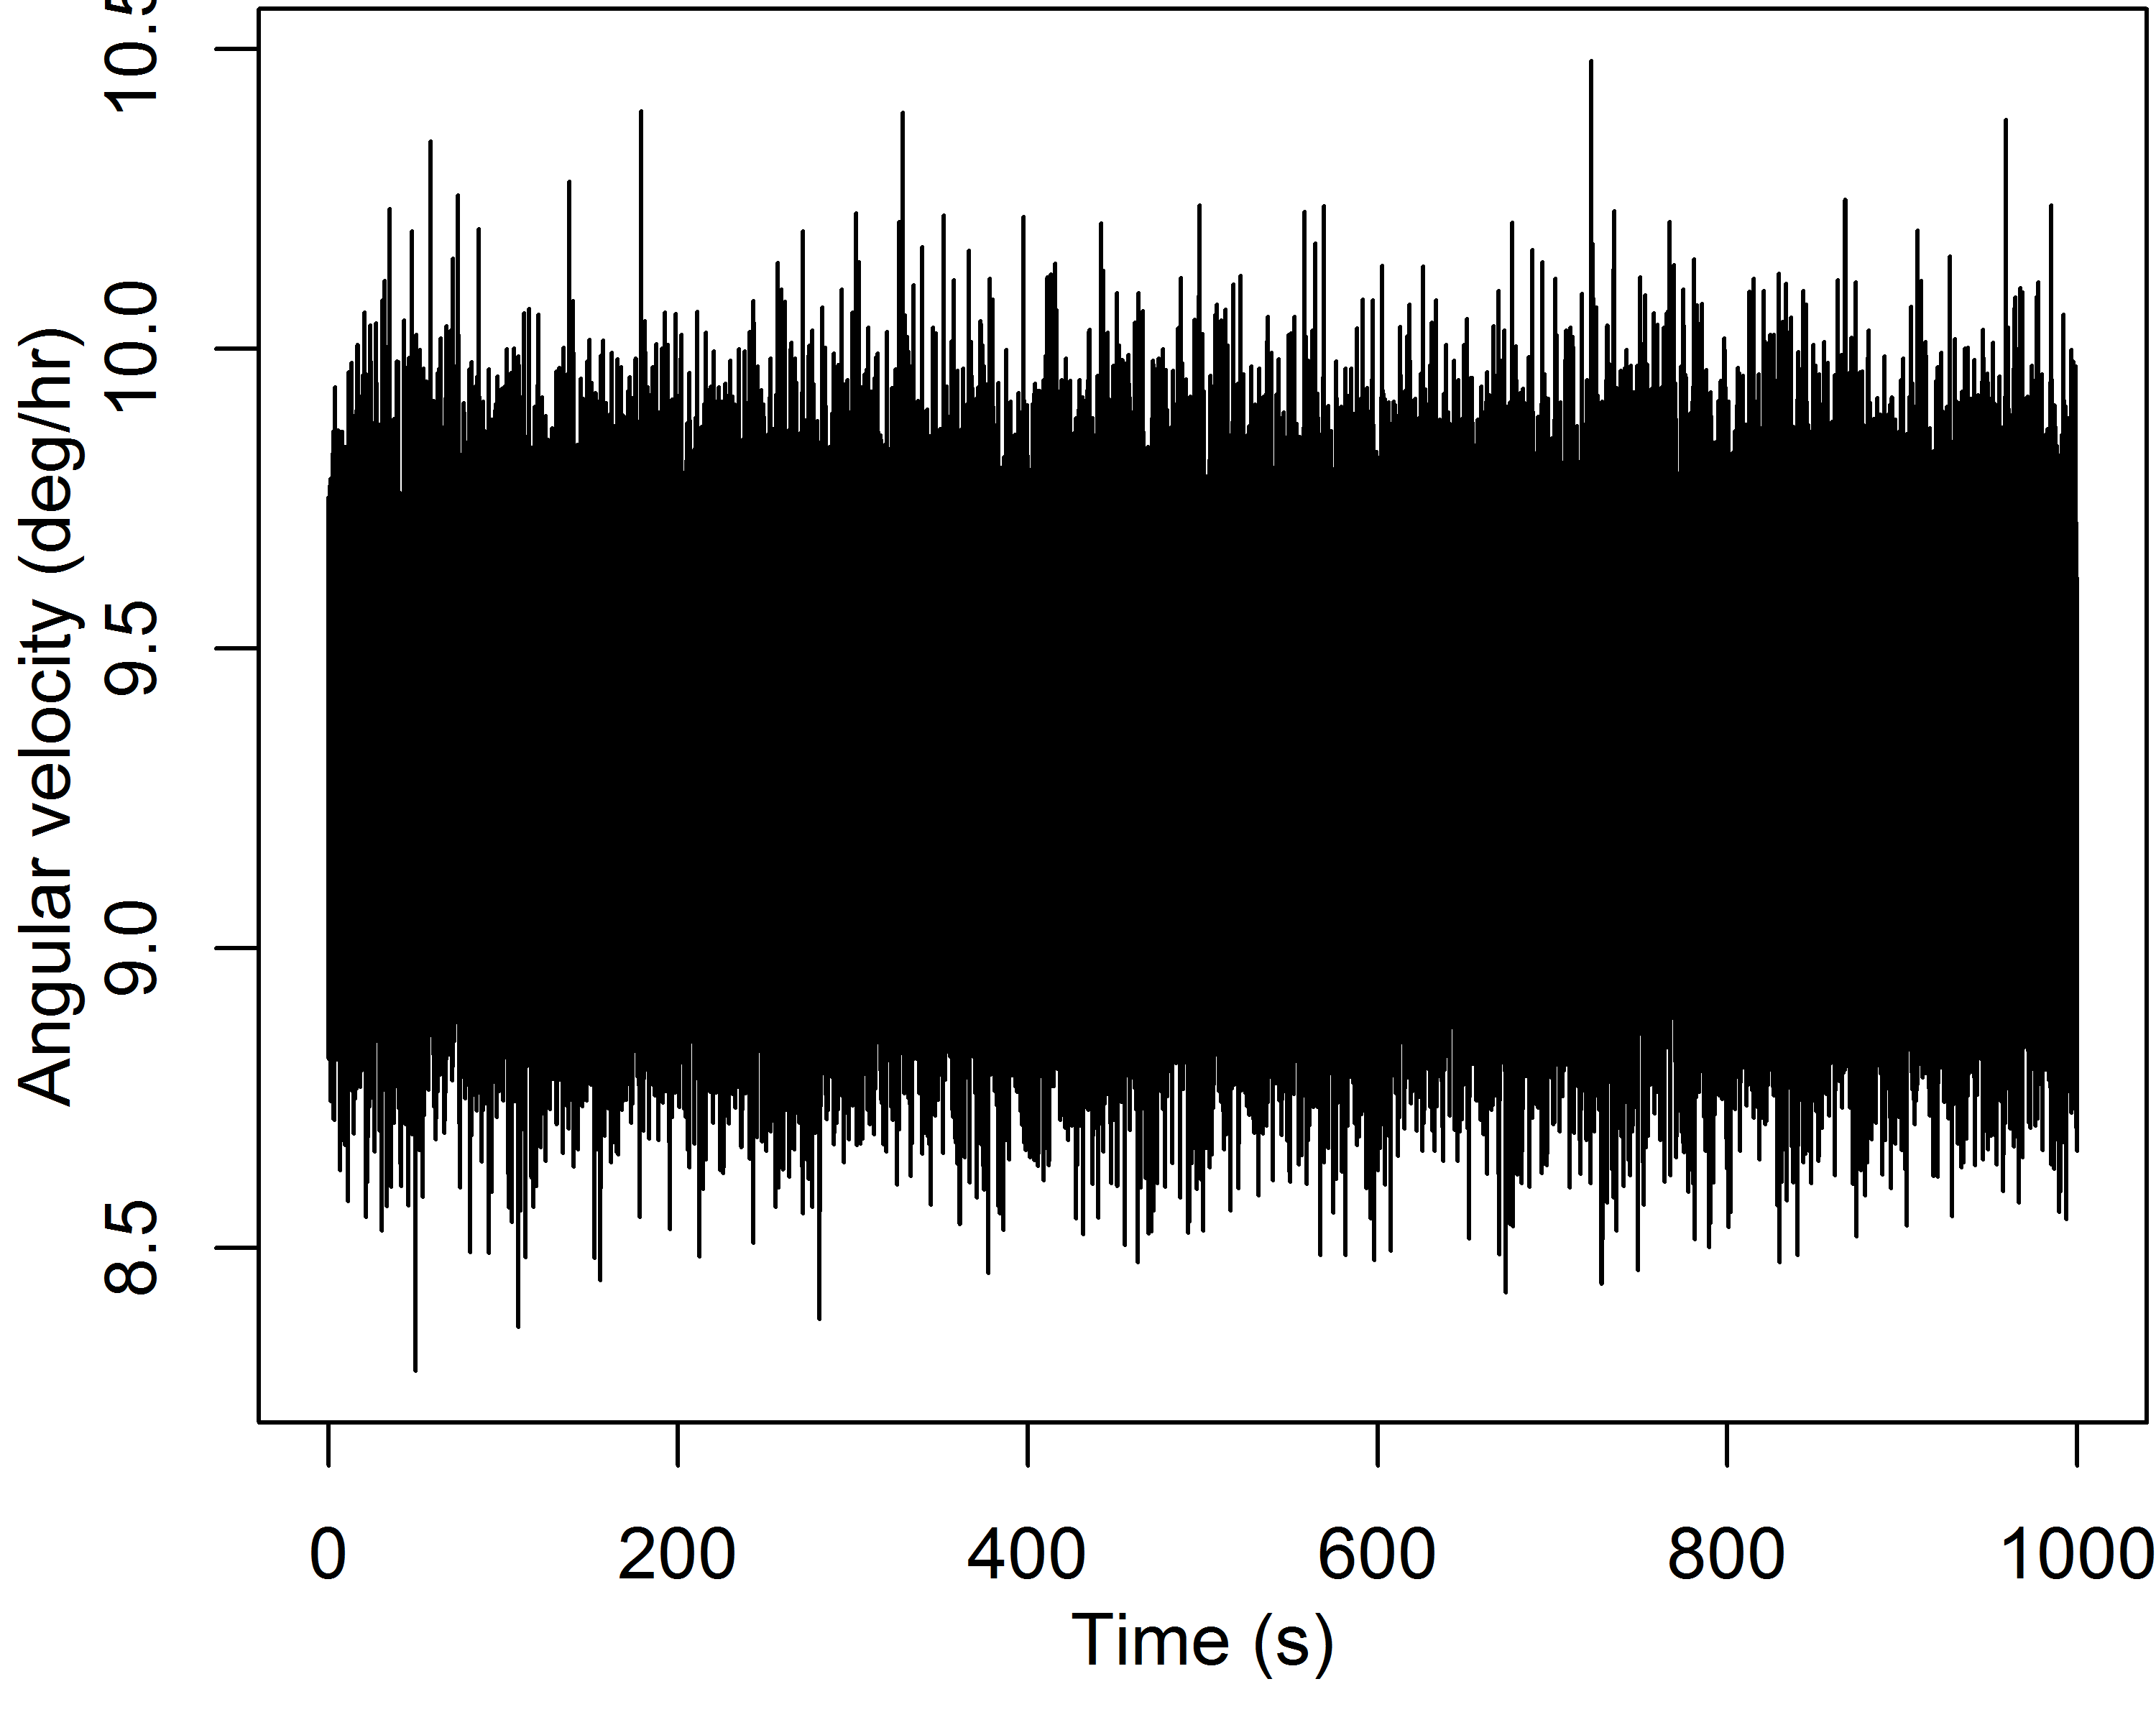
\includegraphics[width=0.98\textwidth]{Figures/snapshot_11005.png} 
		\caption[\SI{1000}{\second} of gyroscope data]{Snapshot of \SI{1000}{\second} of gyroscope data, taken from our \SI{8}{\hour} data sample.}
		\label{fig:snapshot11005}
\end{figure}


The angular random walk (ARW) is a measure of the effects of integrating a noisy velocity measurement. The specification from the manufacturer is ARW = \SI{5e-4}{\deg\raiseto{-0.5}\hour}. This means that if we integrate the gyroscope's rate for 1~hour, the $1-\sigma$ uncertainty on our position would be 
$\SI{5e-4}{\deg}\sim\ang{;;1.8}$. For an integration time of 1 second, it would be \ang{;;0.03}. For a single integration time step $\Deltat = \SI{10}{\milli\second}$, it would be \ang{;;0.003}. 

The manufacturer specification gives a maximum bias instability over a wide range of temperatures less than \SI{0.005}{\deg\per\hour}. This represents how much the mean angular velocity is expected to vary. These tests are an attempt to verify these numbers.


\paragraph{Power spectral density}

The usual frequency-domain analysis tool is the power spectral density (PSD). This allows us to spot any frequency peaks in the data, and let us look at the $1/f$ noise behavior, which is the typical low-frequency behavior that indicates drifts in the signal. The \SI{100}{\hertz} data is all we need, as the gyroscope's bandwidth is \SI{50}{\hertz}. Hence, the \SI{2000}{\hertz} data does not contain any more information than the \SI{100}{\hertz}. In fact, while plotting the PSD of the \SI{2000}{\hertz} data, we can see clearly the break at \SI{50}{\hertz} characteristic of a \SI{50}{\hertz} low-pass filter.

\begin{figure}[!ht]
\begin{subfigure}[b]{0.5\textwidth}

		\centering
		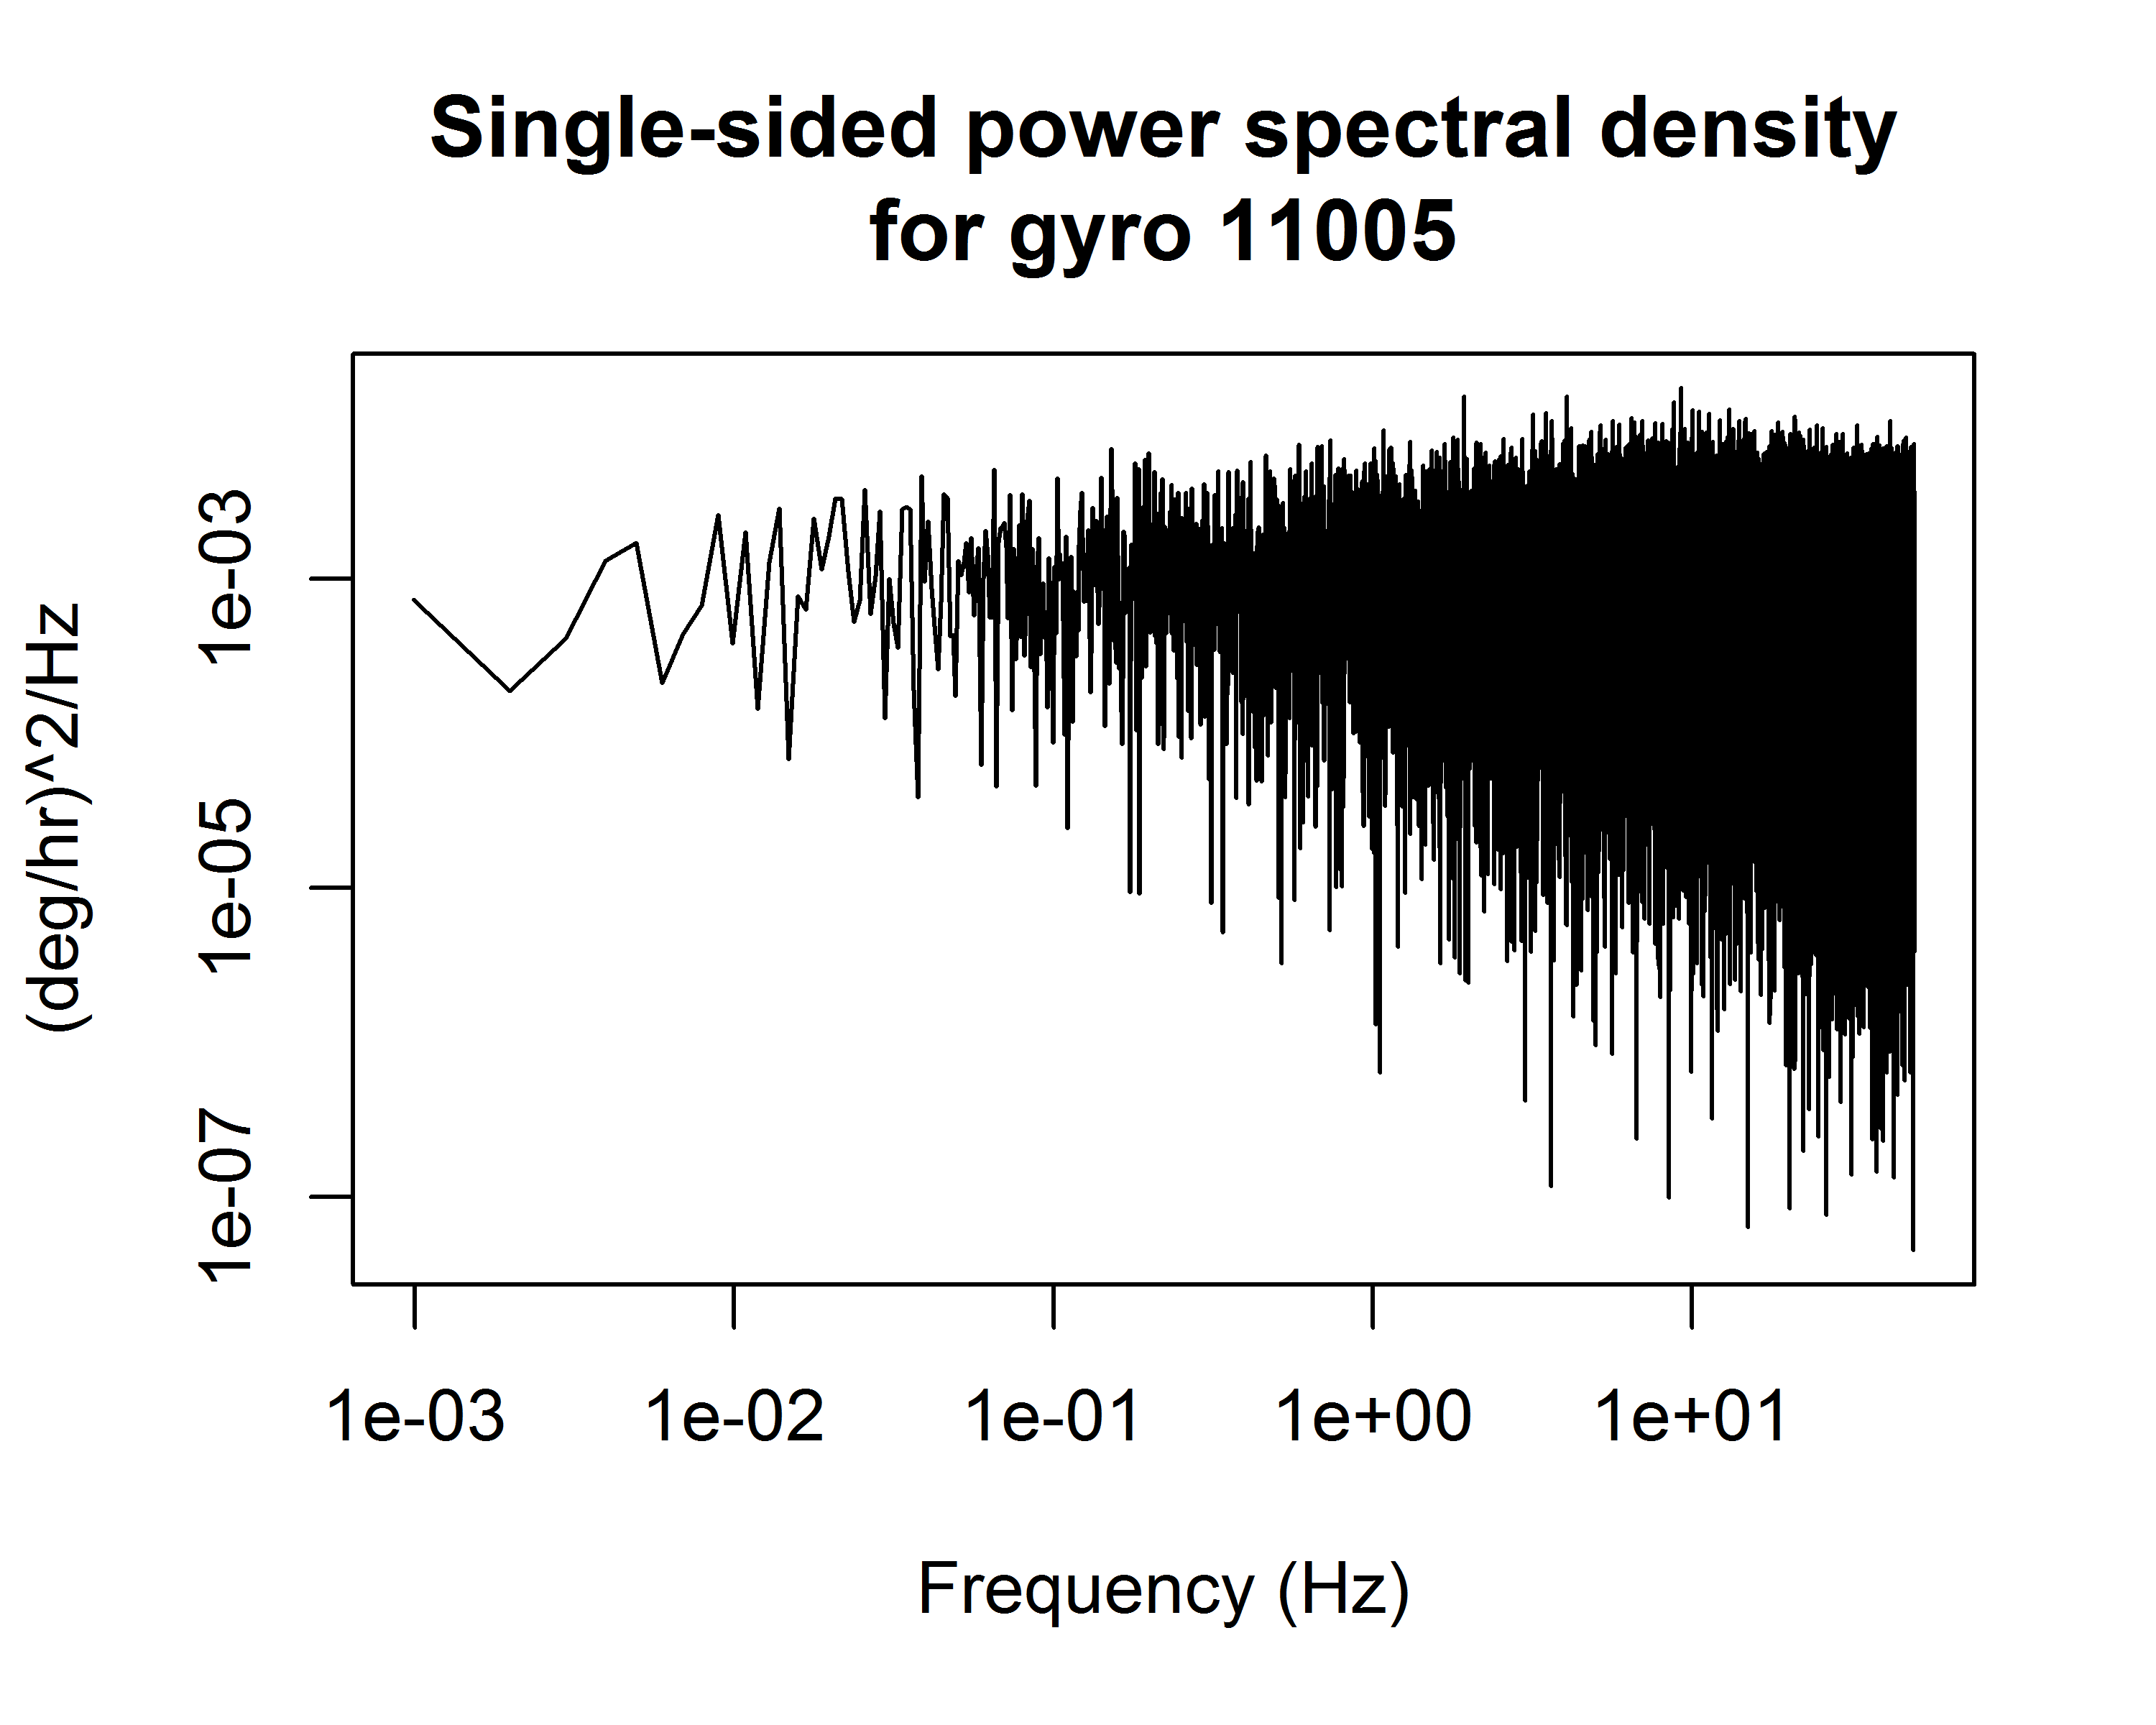
\includegraphics[width=0.98\textwidth]{Figures/sspwsd_11005.png} 
		\caption{}
		\label{subfig:sspsd11005}
\end{subfigure}
\begin{subfigure}[b]{0.5\textwidth}
		\centering
		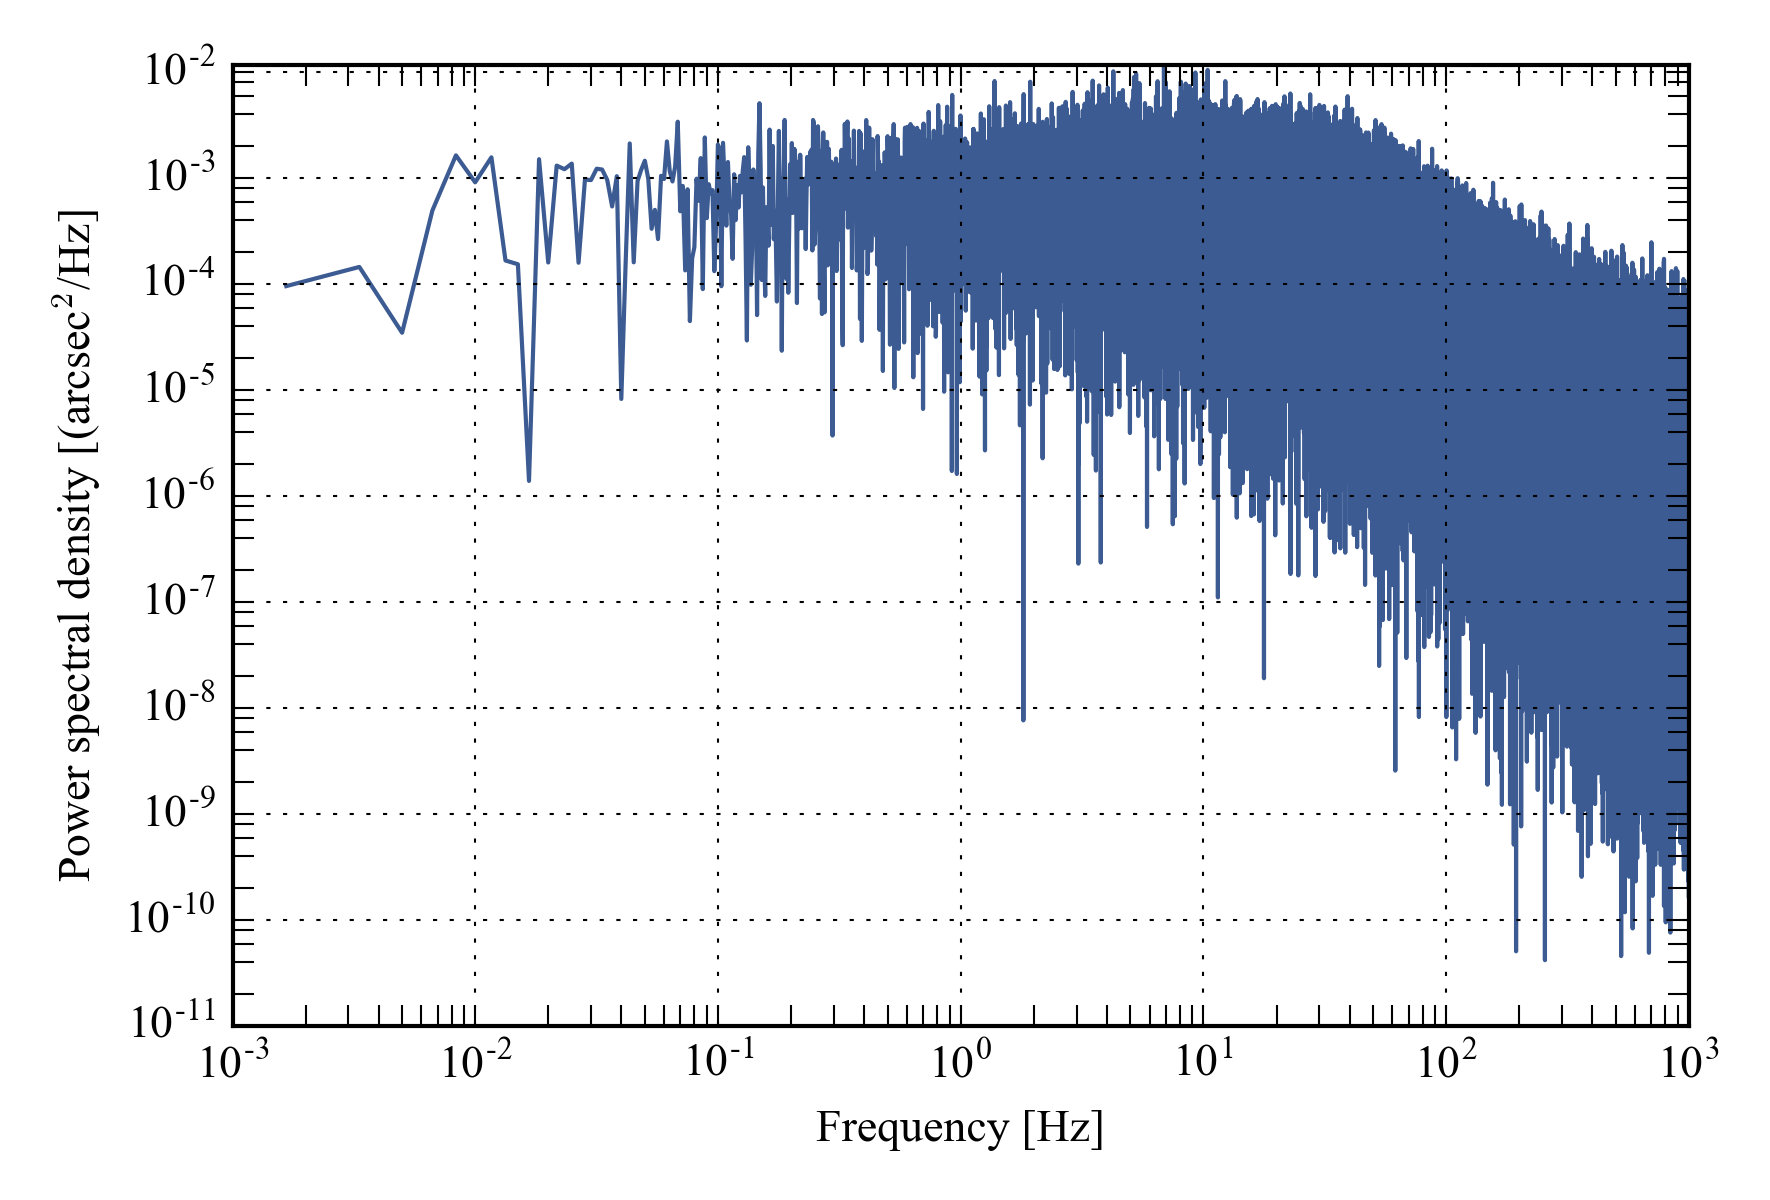
\includegraphics[width=0.98\textwidth]{Figures/sspwsd2000_11005.png} 
		\caption{}
		\label{subfig:sspsd2000-11005}
\end{subfigure}
\label{fig:gyrospectra}
\caption[Power spectral density]{(\subref{subfig:sspsd11005}): Single-sided power spectral density for gyro 11005, an \SI{8}{\hour} sample with a sampling rate of \SI{100}{\hertz}, showing no particular feature (large peaks or resonances). (\subref{subfig:sspsd2000-11005}): Single-sided power spectral density for gyro 11005, a \SI{10}{\minute} sample with a sampling rate of \SI{2000}{\hertz}, showing no electronic resonance peak or other feature. We can notice the \SI{-3}{\decibel} break at around \SI{50}{\hertz}.}
\end{figure}

It is important to note that in their factory settings, the gyroscopes' noise distribution was not normal at all. It exhibited electronic peaks with many harmonics, at frequencies that were varying as a function of the gyroscope inclination (as it was measuring different components of the Earth's rotation). After talking to the manufacturer, we determined that it was caused by the closed-loop algorithms inside the gyroscope electronics. The problem was known by them, and the remedy was to inject a random phase perturbation in the closed loop. This had the effects to get rid of those frequency peaks, at the cost of increasing the overall noise variance by a factor of 4. The noise levels that are specified by the company are very close to the noise seen when using that random phase modulation. Hence, if one does not care as much at the frequency content of the gyroscope, it is possible that this device could work even much better than it does for us.


\begin{figure}[!ht]

\begin{subfigure}[b]{0.5\textwidth}
		\centering
		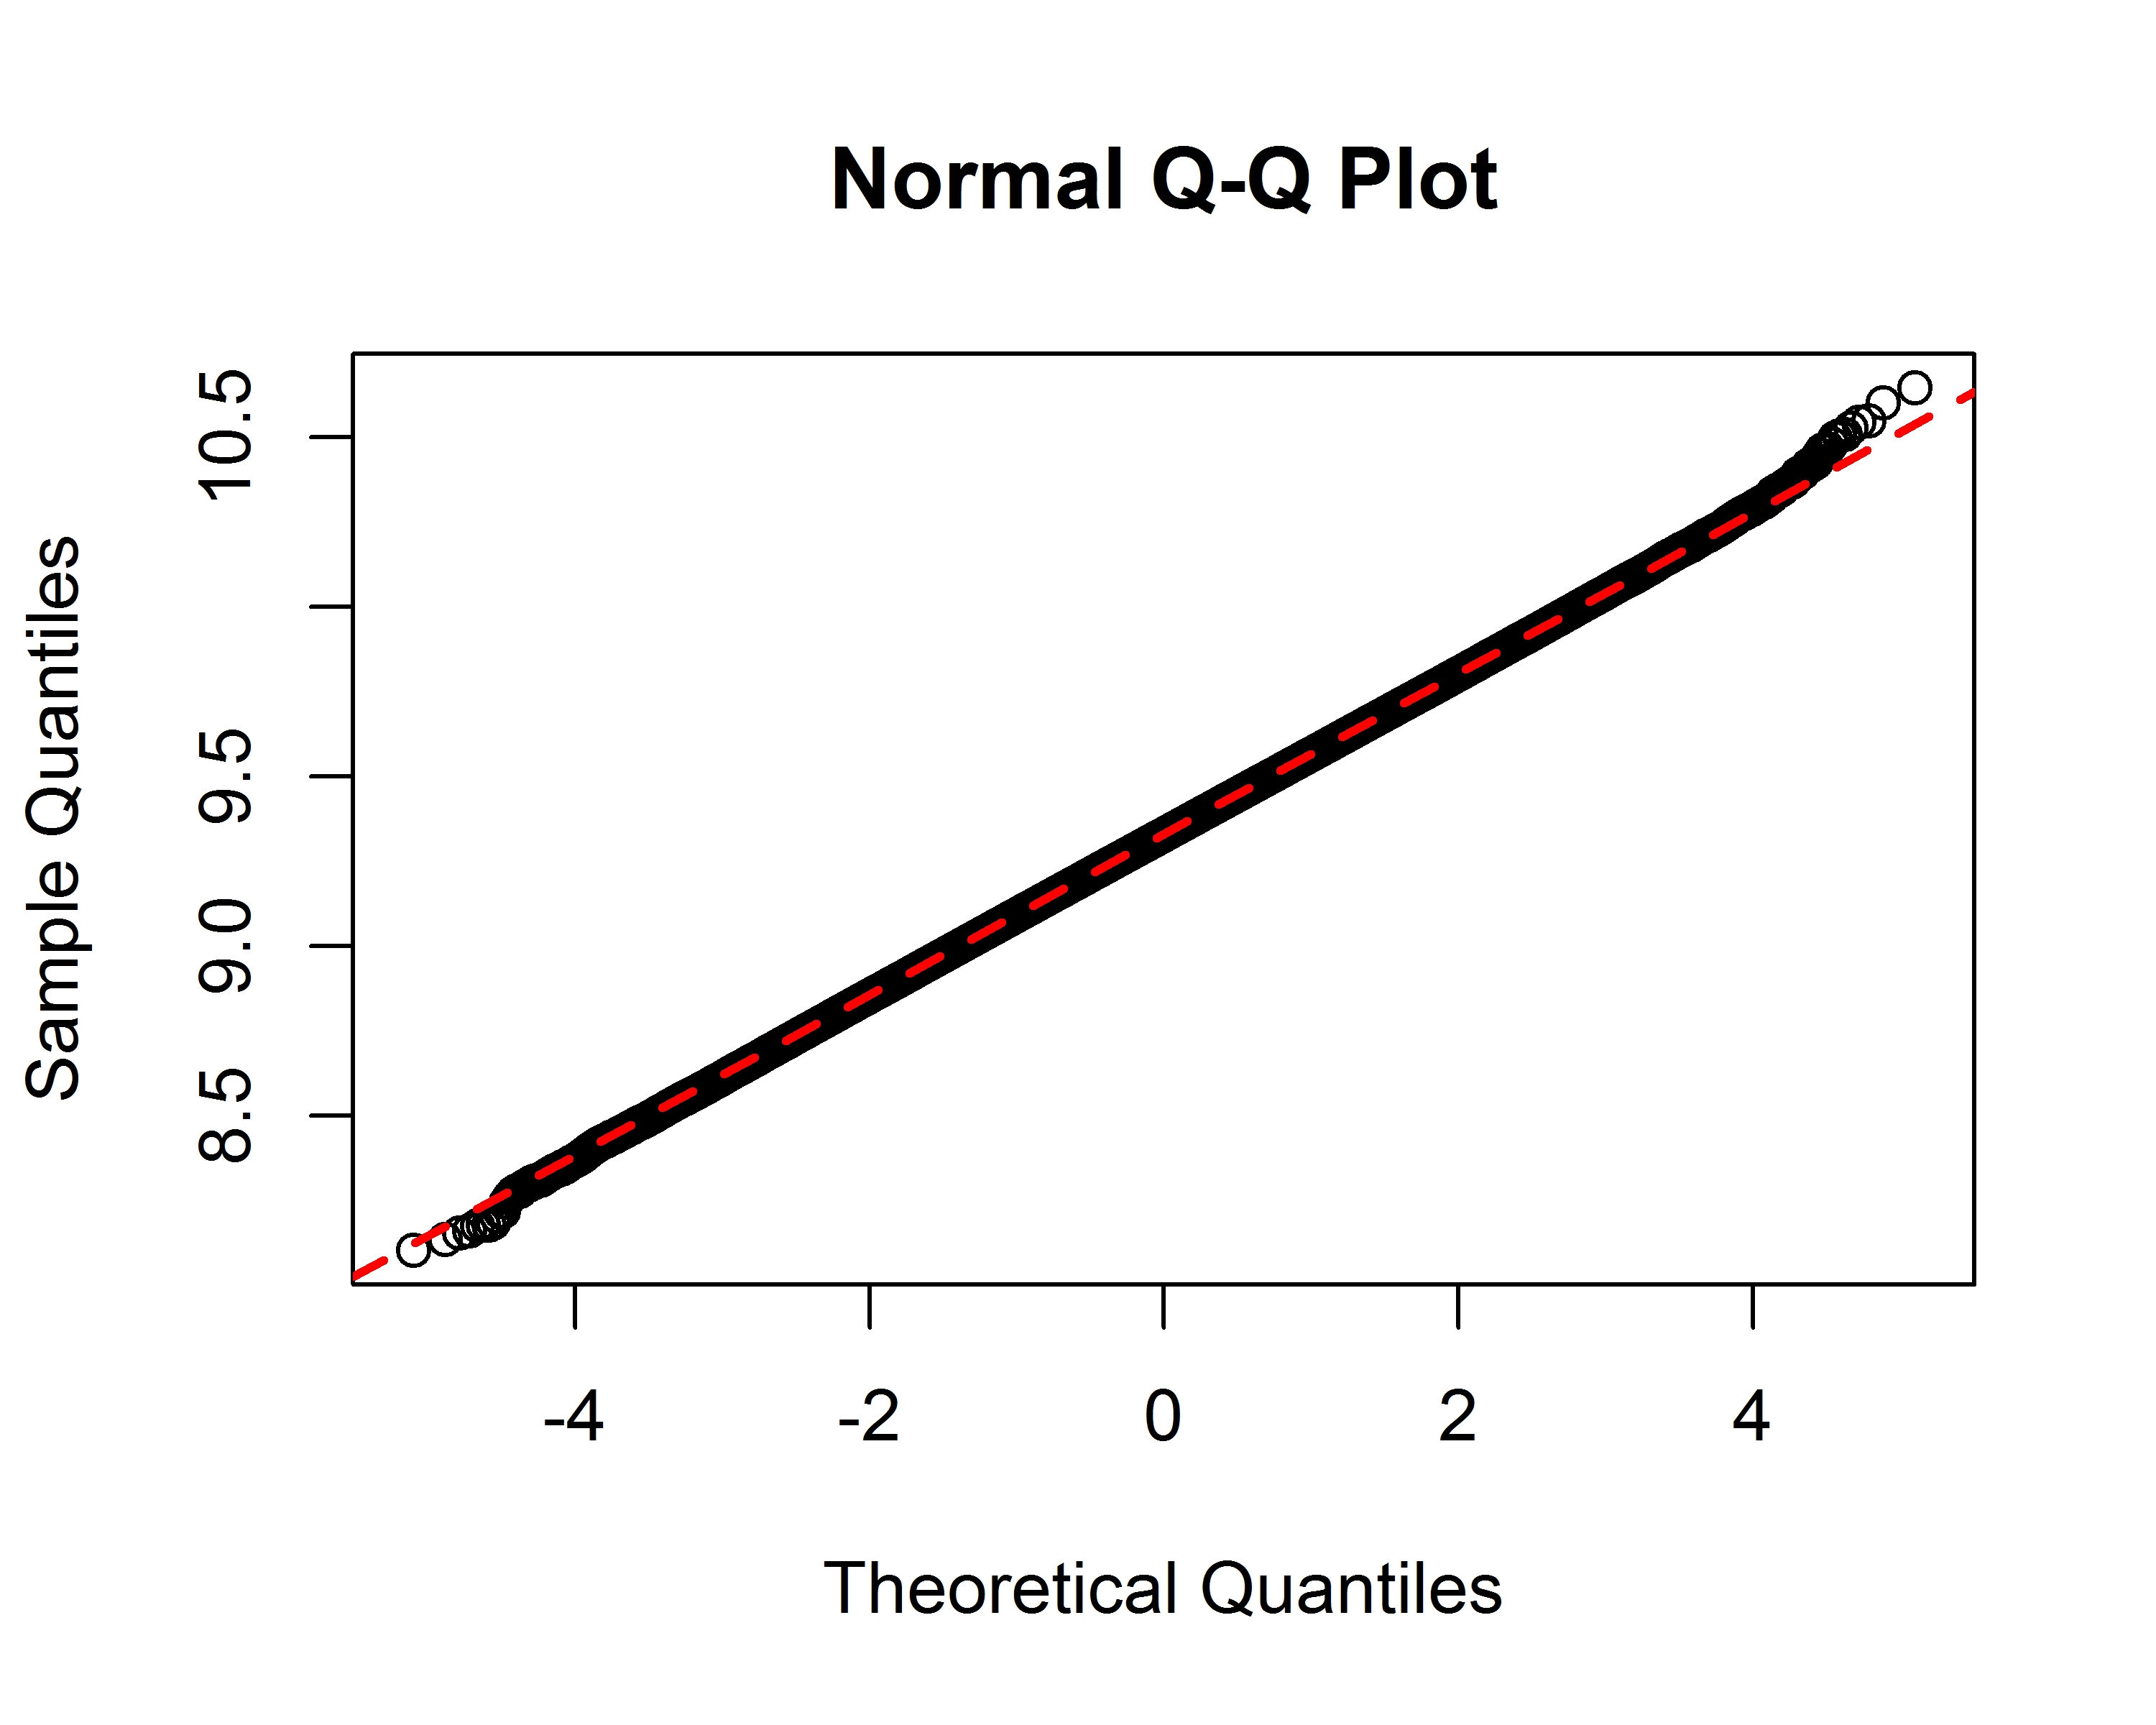
\includegraphics[width=0.98\textwidth]{Figures/qqplot_11005.png} 
		\caption{}
		\label{subfig:probplot11005}
\end{subfigure}
\begin{subfigure}[b]{0.5\textwidth}
		\centering
		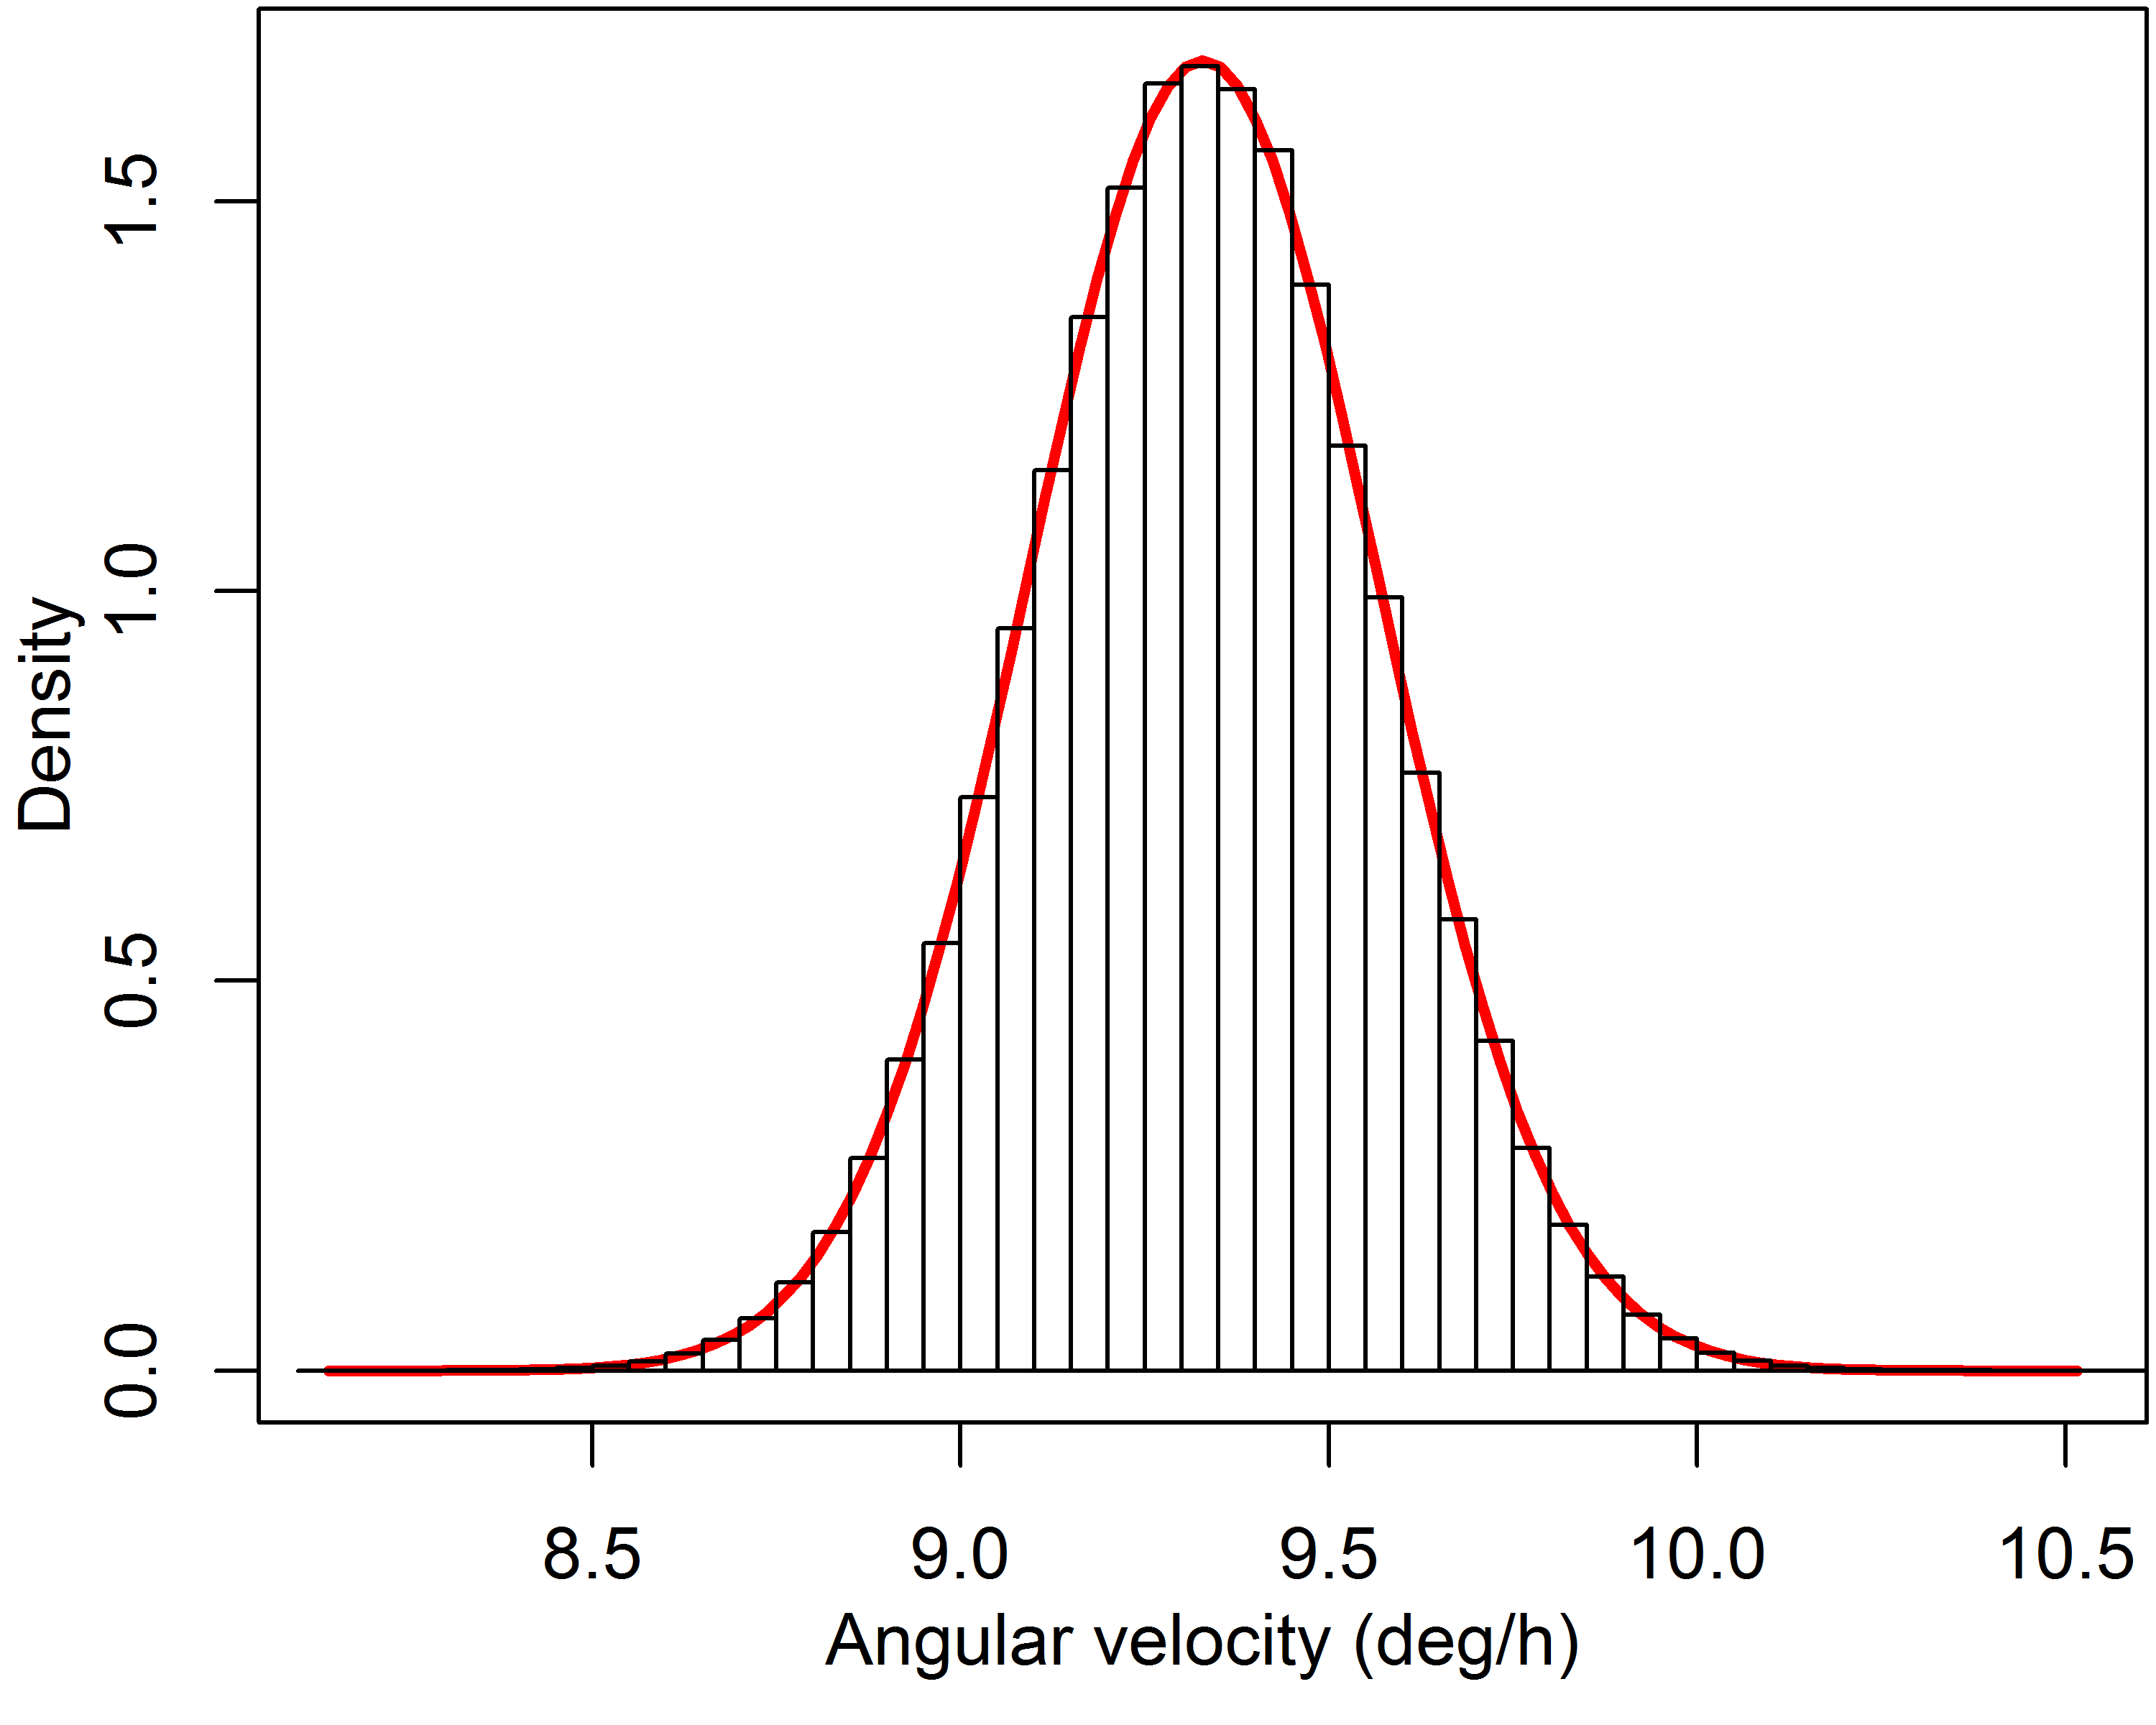
\includegraphics[width=0.98\textwidth]{Figures/distrib_11005.png} 
		\caption{}
		\label{subfig:density11005}
\end{subfigure}
\caption[Normality analysis]{Normality analysis of the gyroscope signal over \SI{8}{\hour} of data taken at \SI{100}{\hertz}. (\subref{subfig:probplot11005}): Normal quantile-quantile plot for an \SI{8}{\hour} sample with a sampling rate at \SI{100}{\hertz}. Here the measured quantiles (fraction of the measured values under a certain value) are plotted against the theoretical quantiles from a normal distribution. The red line is the theoretical distribution if the data were taken from a normal distribution. (\subref{subfig:density11005}): Probability density distribution for an \SI{8}{\hour} sample with a sampling rate at \SI{100}{\hertz}. In red, the theoretical normal distribution we obtain with the measured mean and standard deviation from the sample. While the data is not strictly normally distributed, we consider that it is sufficiently close to a gaussian distribution.}
\label{fig:gyroprobdensity}
\end{figure}

\paragraph{Normality tests}

We ran a few standard normality tests on chunks of the 8-hour data for each gyroscope. While the tests on individual small chunks of data never reject the null hypothesis (that the distribution is normal), the distribution of the total 8 hours does with a very high probability, using both the Anderson-Darling and the Kolmogorov-Smirnov test. It means that it is extremely unlikely that the measured noise over \SI{8}{\hour} is coming from a normal distribution.

Since the data is always consistent with being normally distributed over timescales of tens of minutes, after close inspection of the long-term quartile plots and histograms, we determined that it would be safe to consider the distribution as normal for the purpose of our attitude estimator (see Fig.~\ref{fig:gyroprobdensity}). 




\paragraph{Allan variance}


Another common tool to study of the gyroscope's performance is to plot the Allan variance. The Allan variance gives a time-domain analysis of the gyroscope's noise that is complementary to the power spectral density.

The gyroscopes were successfully tested in the environmental chamber, with no noticeable change in performance except a much larger power draw, due to the Peltier element maintaining the fiber temperature.


\renewcommand{\arraystretch}{1.5}
\begin{table}[htbp]
\small
\begin{tabular}{p{5.5cm}p{2.5cm}p{2.5cm}p{2.5cm}}
\toprule
Measured property & Gyro \#11005 & Gyro \#12003 & Gyro \#12004\\
\midrule
Standard deviation (\si{\deg\per\hour}) & 0.237 & 0.199 & 0.217\\

Angular random walk (\si{\deg\raiseto{-0.5}\hour}) & \num{4.31e-4} & \num{3.79e-4} & \num{4.02e-4}\\

Bias instability (\si{\deg\per\hour}) & \num{3.11e-4} & \num{1.8e-3} & \num{3.05e-4} \\
\bottomrule
\end{tabular}
\label{tab:gyroproperties}
\caption[Gyroscope properties]{Properties of the gyroscopes determined from the Allan variance analysis on an \SI{8}{\hour} sample with a sampling rate at \SI{100}{\hertz}. Note that \SI{1}{\deg\per\hour} =  \SI{1}{\arcsec\per\second}, and the Earth rotates at about \SI{15}{\arcsec\per\second} about the line joining the two poles.}
\end{table}



\begin{figure}[!ht]

	\begin{subfigure}[b]{\textwidth}
		\centering
		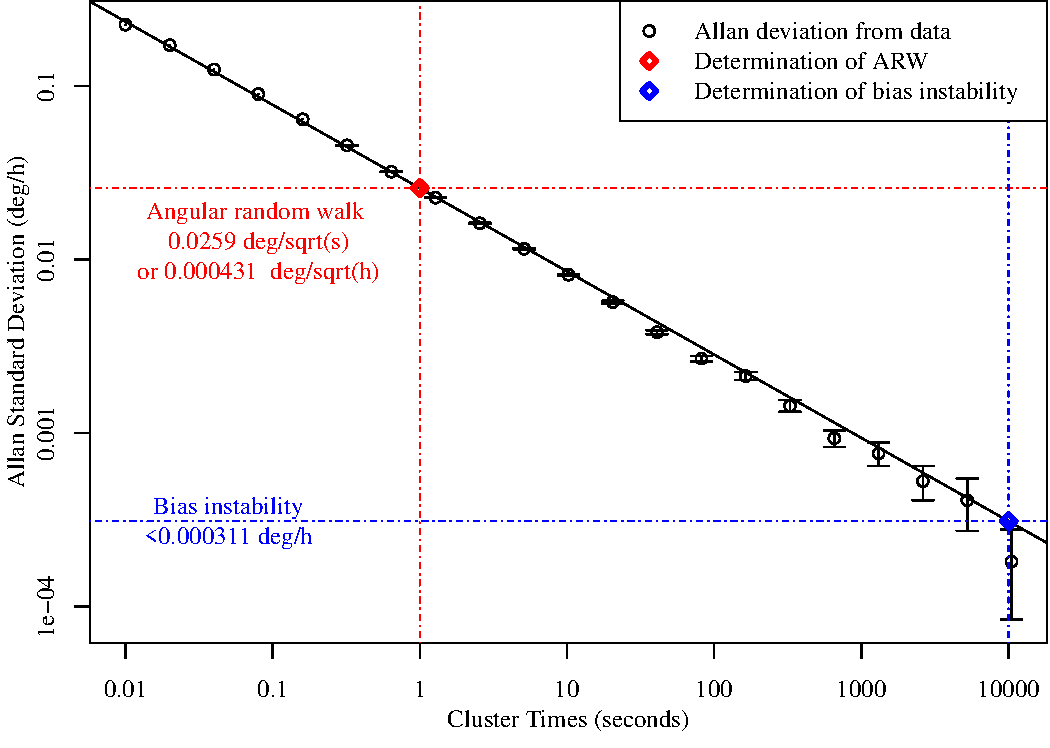
\includegraphics[width=0.98\textwidth]{Figures/allandev_11005.pdf} 
		\caption{Allan deviation of gyro 11005}
		\label{subfig:allan11005}
	\end{subfigure}
	
	\begin{subfigure}[b]{0.5\textwidth}
		\centering
		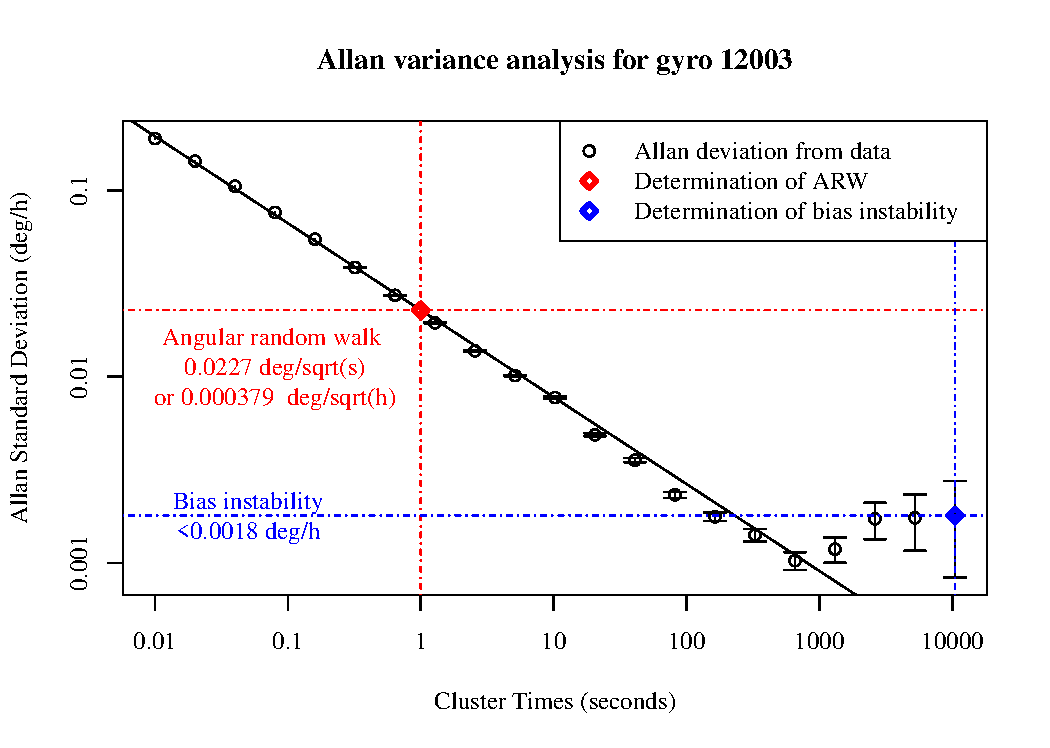
\includegraphics[width=0.98\textwidth]{Figures/allandev_12003.pdf} 
		\caption{Allan deviation of gyro 12003}
		\label{subfig:allan12003}
	\end{subfigure}
	\begin{subfigure}[b]{0.5\textwidth}
		\centering
		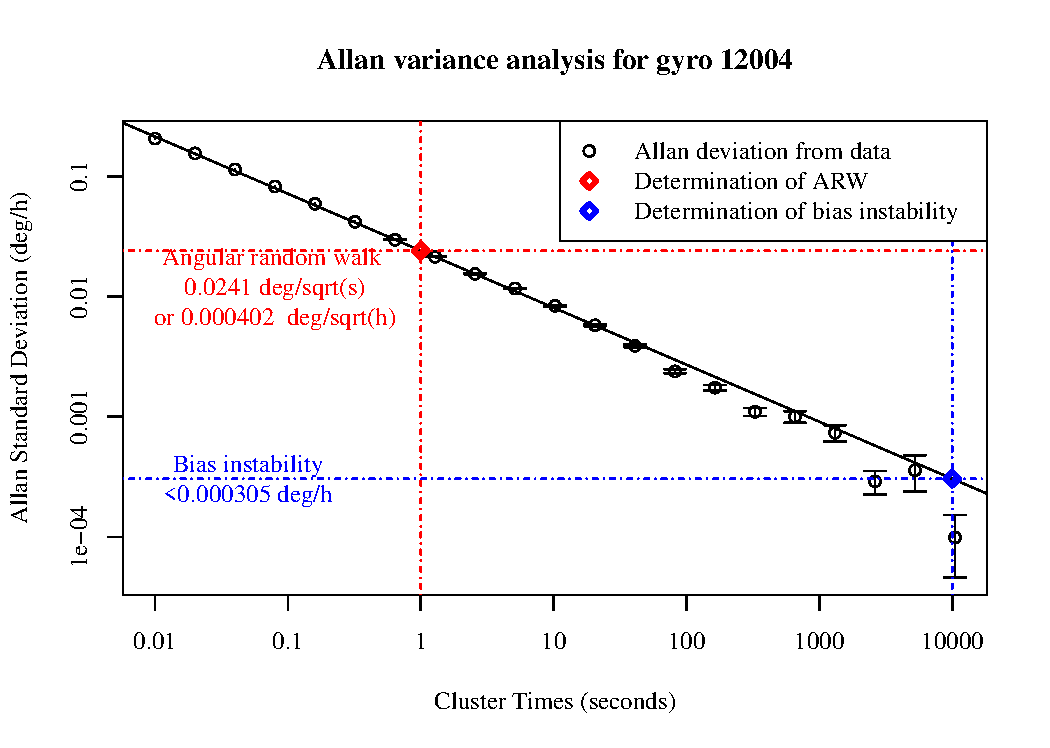
\includegraphics[width=0.98\textwidth]{Figures/allandev_12004.pdf} 
		\caption{Allan deviation of gyro 12004}
		\label{subfig:allan12004}
	\end{subfigure}

\end{figure}

\paragraph{Gyro unit alignment}



\subsubsection{Star cameras}

We have designed, built and tested a custom star camera setup that provides higher accuracy measurements than commercially available devices. Our collaborators from Cardiff University provided the star camera software, which solves for the inertial orientation from a given picture. This software is a C++ set of routines that was originally developed for the EBEX balloon experiment \citep{Oxley:2004hl}. 

Our star camera design features an old-generation Nikon Nikkor \SI{300}{\mm} f/2.8 telefocal lens with manual focus and extended hood. These lenses were manufactured between 1977 and 1982 and can be found today online through websites like e-Bay. The lens provides low chromatic aberration, a magnification of \SI{688}{\arcsecond\per\mm}, a wide field of view ($\approx$~\SI{10}{\degree}) and a collecting area of \SI{90}{\mm\squared} which is is larger than most star tracking assemblies. This old lens does not feature a built-in autofocus or any of the image stabilization actuators commonly found in modern lens assemblies: these could have become a liability in the severe balloon environment. 

Our camera is a USB3.0 Point Grey Grasshopper3. The CCD is a Sony Pregius IMX174 CMOS sensor with 1920$\times$1200 pixels at \SI{5.86}{\um} pitch. This provides a field of view of \SI{2.14}{\degree}$\times$\SI{1.34}{\degree} and a pixel scale of \ang{;;4.02}/pixel. It features a very convenient software suite which works with all the Point Grey camera products, and leaves room for future potential upgrades of the camera. The detector characteristics are summarized in Table~\ref{tab:starcamproperties}.

\renewcommand{\arraystretch}{1.5}
\begin{table}[htbp]
\label{tab:starcamproperties}
\small
\begin{tabular}{p{4cm}|p{1cm}|p{8.5cm}}
\toprule
Property & Value & Description \\
\midrule
Quantum efficiency at \SI{525}{\nm} (\%) & 76 & Fraction of incoming photons that create signal \\

Read noise (electrons) & 6.83 & Error made when reading the pixel's value \\

Absolute sensitivity threshold (photons) & 9.77 & Minimum number of photons required to get a $\SNR=1$ on a pixel\\

Well depth (electrons) & \num{32513} & Maximum number of electrons a pixel can store\\
\bottomrule
\end{tabular}
\caption[Star camera properties]{Star camera properties}
\end{table}



We have successfully cycled the camera in the environmental chamber all the way until the camera's internal thermometer indicated a temperature of \SI{-80}{\celsius}, and it continued operating fine.

\paragraph{Focusing strategy}
Focusing the camera could be required at float due to the change in temperatures that could create a shift of the focal plane. We implemented our own autofocus mechanism, a belt is attached between the lens' focus ring and a stepper motor. When the stepper motor turns, it turns the focus ring. We tested this very simple configuration in our environmental chamber only to realize that the belt was loosing grip when the temperature was too cold. To fix this problem, we added a spring-based belt tensioner which adds a $\approx$~\SI{20}{\newton} of force to the belt.

At cold temperature and low pressure, we noted that the glass in the lens began to exhibit radial cracks, presumably caused by the CTE difference between the steel housing and the glass material. These cracks don't noticeably affect image quality, but of course they could cause the glass to shatter if they become too large. Hence, it was decided to maintain the outside temperature of the lens above \SI{0}{\celsius} at all times during flight.

\begin{landscape}
\begin{figure}[!ht]
	\centering
	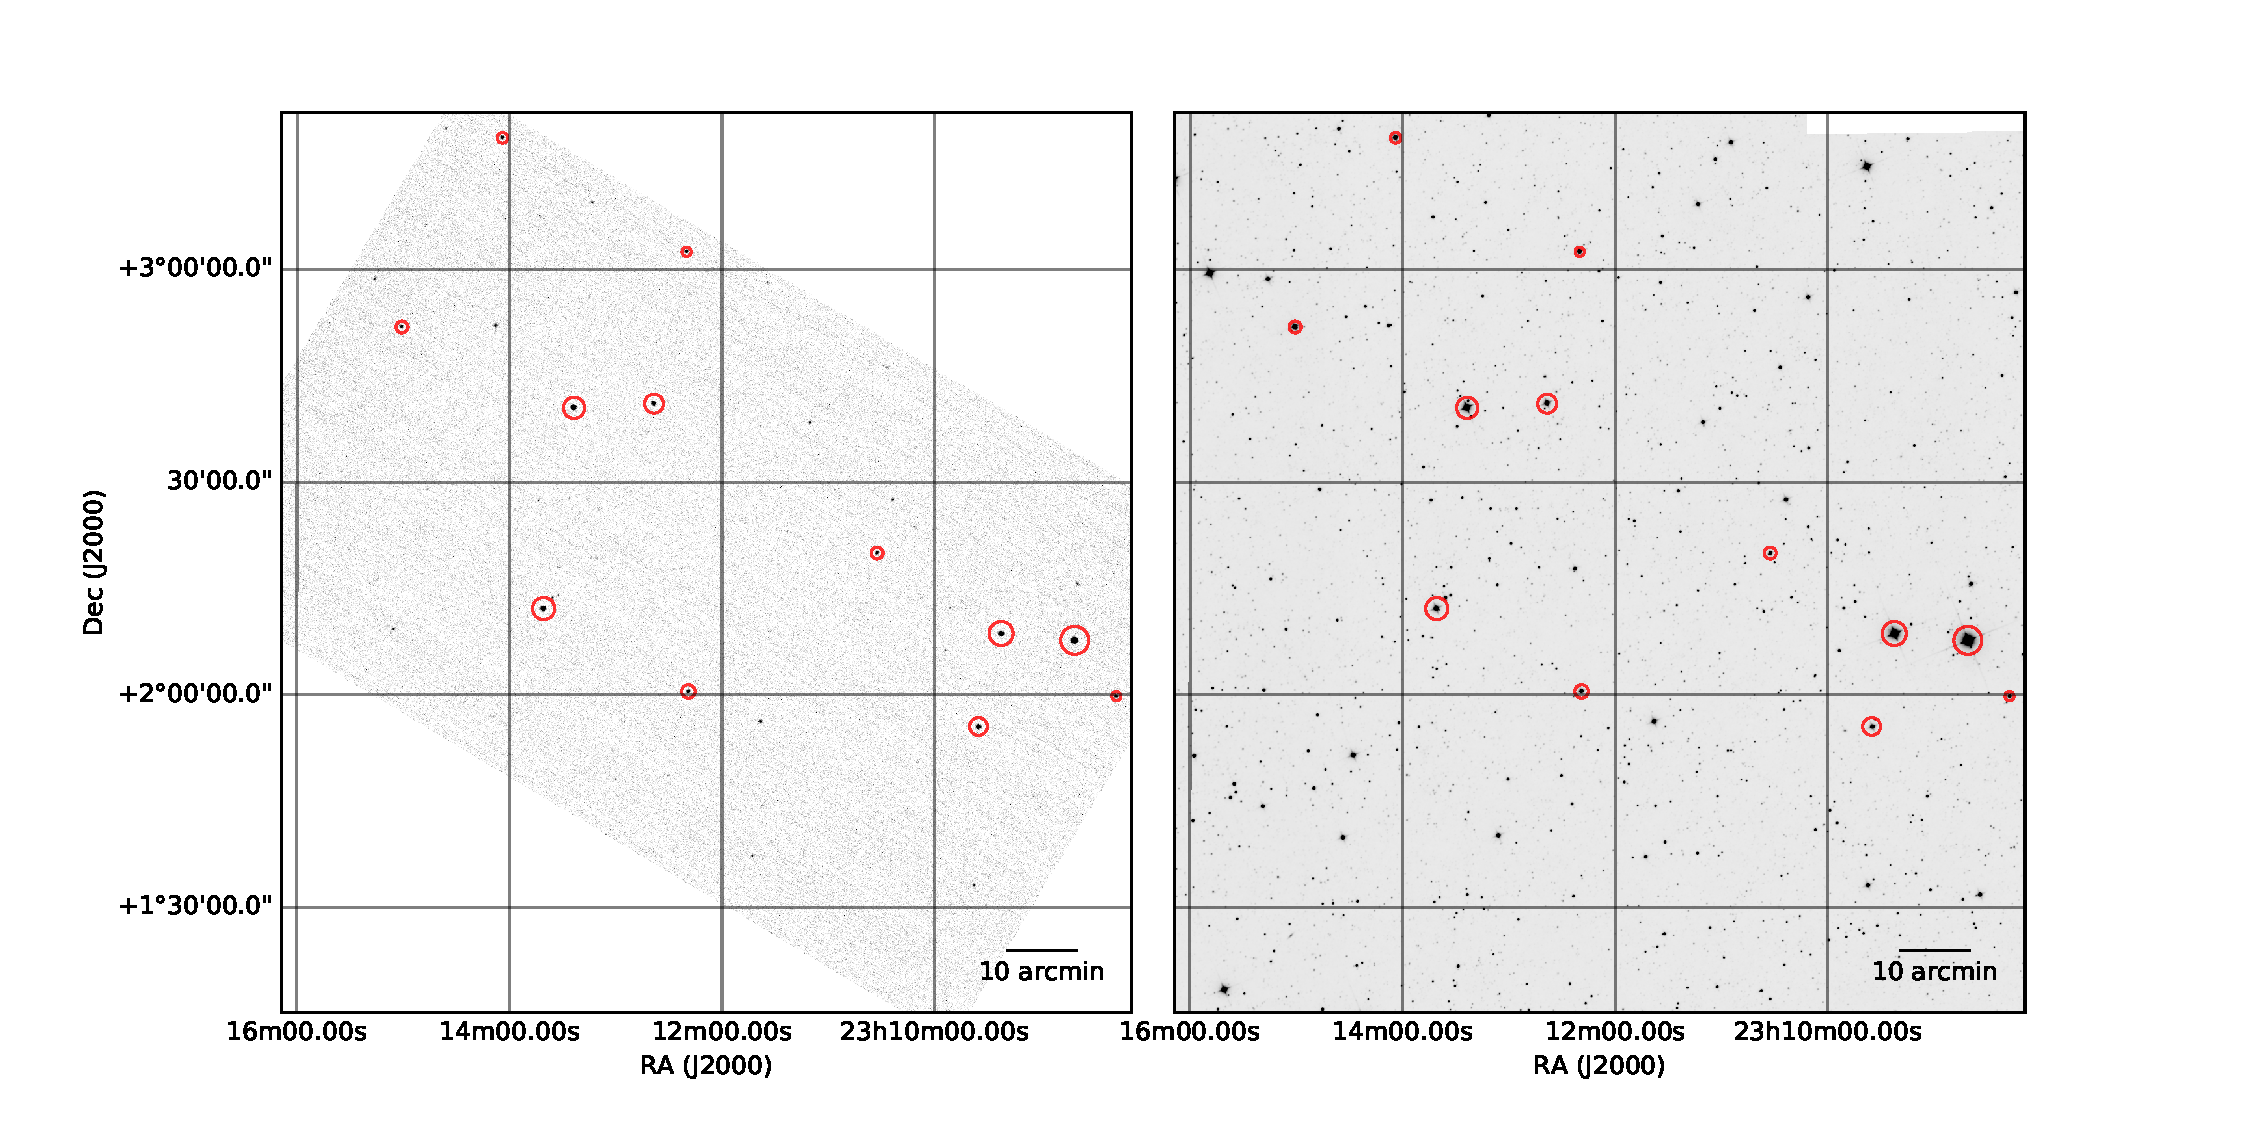
\includegraphics[width=1.5\textwidth]{Figures/starcam_images.pdf}
	\caption[Star camera example WISE]{\textit{Left}: Example of a background-subtracted star camera image with identified $>5\sigma$ sources circled in red. The orientation of the image on the celestial sphere is the one provided by BETTII's embedded star camera solver. This image corresponds to a field in the Scorpius constellation. \textit{Right}: WISE \SI{3.4}{\um} mosaic from the online archive, centered on the same location. This image is composed of 9 individual WISE images that we patched into a mosaic using the \textit{Montage}[CITE] software package.}
	\label{fig:starcamexample}
    \end{figure}
\end{landscape}
\begin{landscape}
\begin{figure}[!ht]
	\centering
	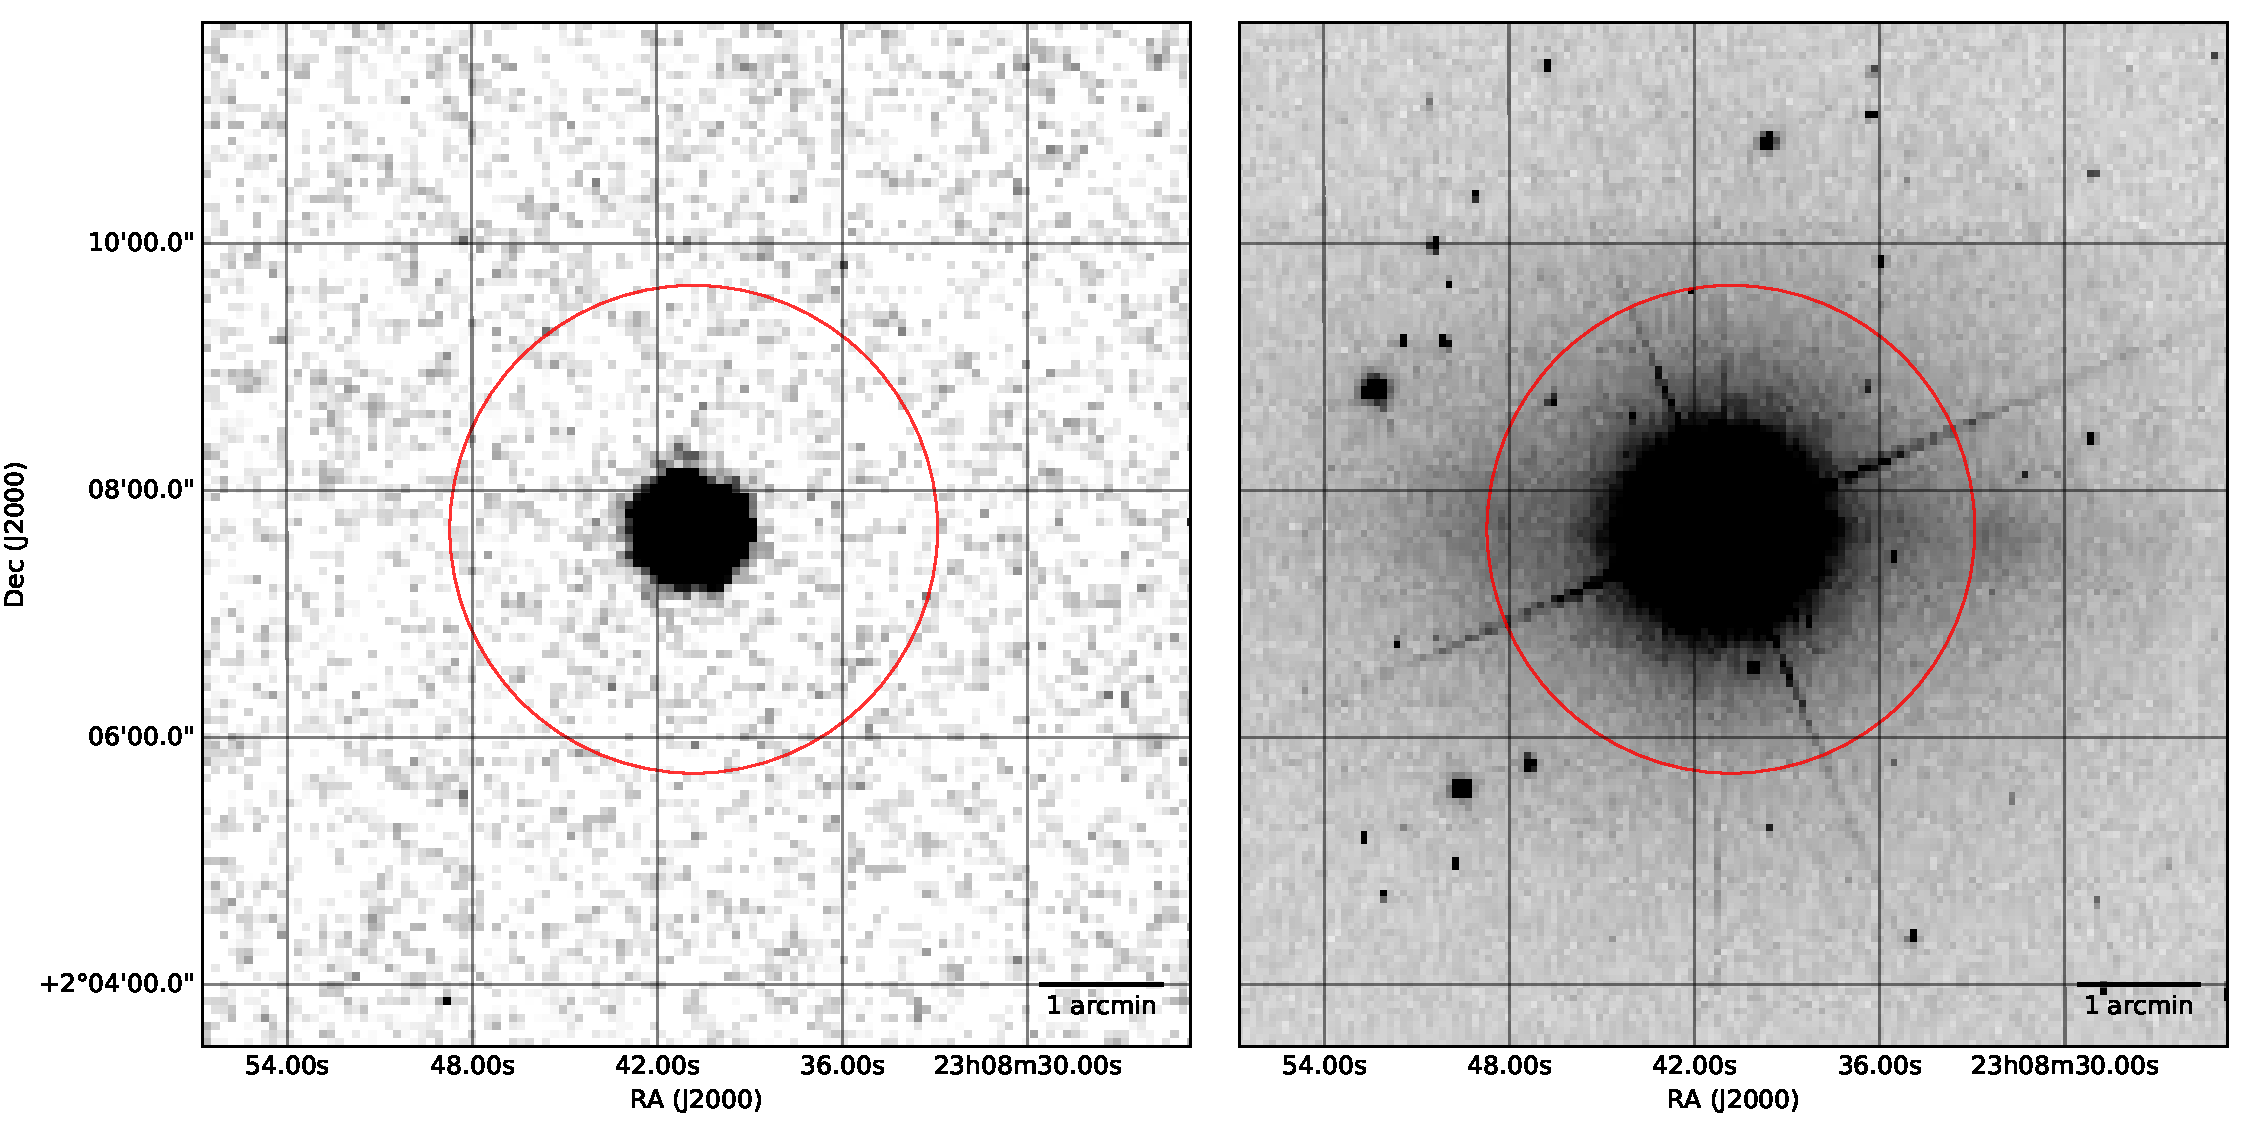
\includegraphics[width=1.5\textwidth]{Figures/starcam_SDSSr_zoom.pdf}
	\caption[Star camera individual star]{\textit{Left}: Snapshot of a bright star seen within the background-subtracted star camera frame. \textit{Right}: Snapshot taken at the same location from the WISE \SI{3.4}{\um} archive.}
	\label{fig:starcamzoom}
    \end{figure}
\end{landscape}

\paragraph{Star camera algorithm tuning}

Talk about the algorithm and its tuning: bandpass filter; field of view; new BETTII catalog;
\subsubsection{Azimuth control (CCMG)}

The CCMG features multiple encoders and motors. First, there is a brushless DC motor that spins each wheel, with a relative 13-bit encoder that monitors where the wheel is in its rotation. Second, there is a Beckhoff AS1050 stepper motor that controls the wheels' shaft angle. On the gimbal, there is a 13-bit  absolute magnetic encoder that measures the angle of the wheels from some reference. 

The motion controller that we use to monitor the wheel's speed is a brushless-DC Galil motion controller DMC-4020. It reads out the wheel encoders and controls the current to the wheels accordingly. It directly, independently implements the closed-loop system of the wheels, including all of the gains, acceleration/deceleration, and jogging speeds associated with the desired motion.

The motion controller was modified to accept an external clock pulse in order to synchronize the wheels' motion with our master clock signal. It requires a clock pulse at \SI{1.024}{\kilo\hertz}, and deviations from this value will require changing some of the gains - it is our understanding that the controller uses a \SI{1.024}{\kilo\hertz} crystal oscillator to generate it's time basis, as some of the gains and parameters to the controller can directly be entered as, for example, "steps per second". 

At power-up, the wheels immediately start accelerating to their cruising speed of \num{3000}~rpm. They take about 10 minutes to reach their target. The wheels' frequency is set for the entire duration of the flight.

The gimbal is controlled with another Galil Motion controller, a 2-axis stepper driver DMC-4020, which can also be synchronized with an external clock. Only one axis is used for the CCMG, while the second axis is used by the momentum dump motor (see section~\ref{subsec:chap3momdumpmotor}). The controller operates in micro-stepping mode and has a very smooth response, in contrast to previous controllers we tested which create a lot of vibrations. The controller is set always to use 64 micro-steps per step, and the motor is a [REFERENCE] with 200 steps per revolution. The motor is outfitted with a Beckhoff AG1000 planetary gearhead with a 3.7:1 reduction ratio. The gearbox itself has a ratio of 25, which creates a total gear ratio of 92.5. Hence, a \SI{360}{\degree} revolution of the stepper corresponds to $360/92.5=3.9^\circ$ motion of the shaft. A motion of \SI{1}{\degree} of the shaft correspond to \num{3889} motion controller steps. A motion of \SI{90}{\degree} of the shaft correspond to \num{296000} motion controller steps. Finally, the same \SI{90}{\degree} motion will translate to a \num{2048} step change in the gimbal magnetic encoder.

In practice, all of the control is done using the regular stepper motor encoder. The magnetic encoder is used for limit-checking and to feed back to the momentum dump mechanism. With this in mind, we can now relate the control signal (stepper motor micro-steps per second) to the physical torque that the wheels provide. 
\begin{eqnarray}
\Delta\theta\units{\si{\radian}} &= &\frac{2\pi}{92.5\times 200\times 64}\Delta(\textrm{micro-steps}) \\ 
& \sim & \num{5.3e-6} \Delta(\textrm{micro-steps})\\
\Delta\theta\units{\si{\arcsecond}} &\sim &  1.09 \Delta(\textrm{micro-steps})
\end{eqnarray}

At \num{3000}~rpm, the CCMG has a total stored momentum $\MCCMG= \SI{20.8}{\newton\meter\second}$. Of course, depending on the orientation of the wheels, the momentum along the $\z$ axis is only the projection of this momentum vector,
\begin{equation}
\MCCMGz\units{\si{\newton\meter\second}} = 20.8\sin\theta,
\end{equation}
where $\theta\units{\si{\radian}}$ is the angle between the horizontal axis and the rotation axis of the wheels. This makes sense: when the wheels are horizontal, there is no momentum projected on the $\z$ axis because the rotation vectors of the wheels are orthogonal to $\z$. When the rotation axes are along $\z$, we have the maximum momentum along $\z$. 

The torque is the variation of the momentum with time. So we can write:
\begin{eqnarray}
\ccmgtorque\units{\si{\newton\meter}} &= &\frac{d}{dt}\MCCMGz\\
\ccmgtorque\units{\si{\newton\meter}} &= & 20.8\times \dot{\theta}\units{\si{\radian\per\second}} \cos\theta\\
 &= & \num{1.1e-4}\times \velstepper\units{micro-step~\si{\per\second}}\cos\theta
\end{eqnarray}

\begin{figure}[!ht]
	\centering
	\includestandalone{Figures/CCMG-nocase-axes}
	\caption{}
	\label{fig:CCMGnocase}
    \end{figure}

\begin{figure}[!ht]
	\centering
	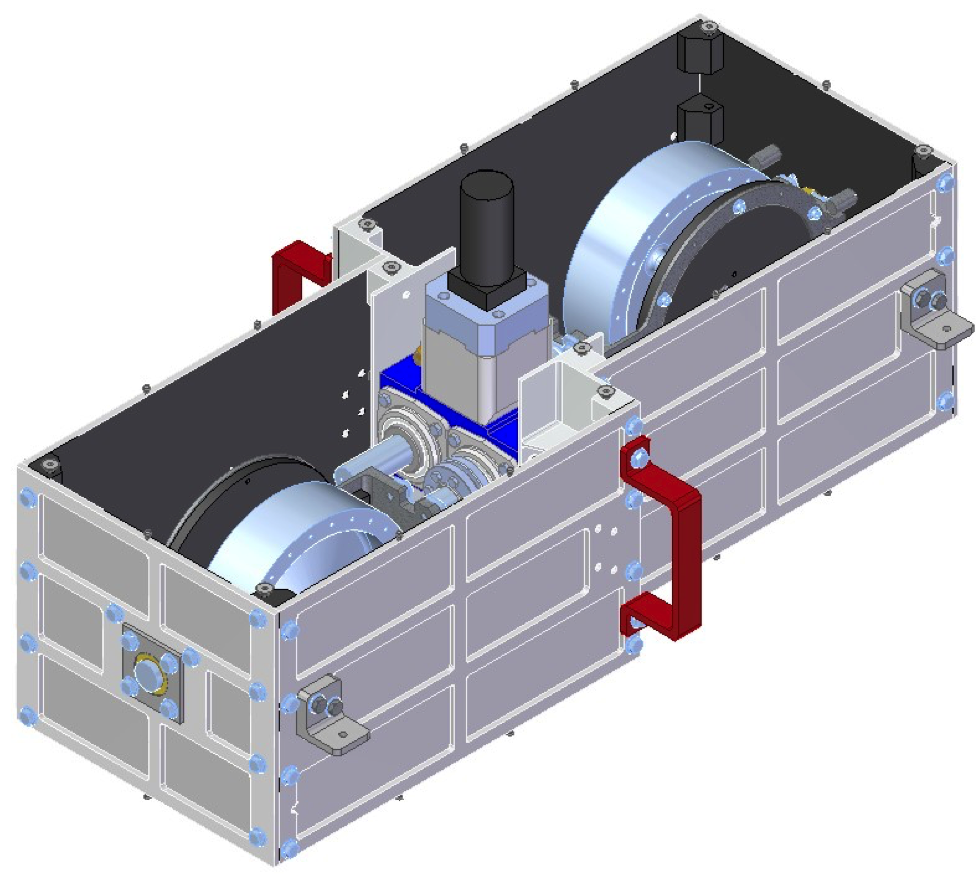
\includegraphics[width=\textwidth]{Figures/CCMG-case.png}
	\caption{}
	\label{fig:CCMGcase}
    \end{figure}


The entire CCMG assembly was tested in a vacuum chamber at cold temperatures, and operates fine. Several heaters are strategically located in the assembly to allow some thermal control for all the electronics in case issues arise.

\subsubsection{Momentum dump mechanism}
\label{subsec:chap3momdumpmotor}

The momentum management strategy consists of using the balloon as a large momentum reservoir. The control system then needs to be equipped with a system that allows a transfer of momentum between the gondola and the balloon, which are connected through the parachute and ladder. 

For this purpose, BETTII uses a design which has successfully flown on previous balloon payload (Fig.~\ref{fig:rotator}), with several improvements over its predecessors. It consists of a steel an titanium setup which will make the junction between to the bottom of the balloon train (at the very bottom of the ladder) and the very top of the gondola. The critical material is an alloy of steel that has been heat treated and is particularly strong. The setup consists essentially of a pivot and a pin made with this allow, connected together with grade 8 bolts. The top of the pin is attached to the pivot, and has a lip at the bottom on which two circular bearings are stacked: the bottom one uses ceramic balls (for their excellent friction properties and long lifetime), and the top one uses steel balls (for their excellent strength). Between the two bearings, there is a metal holder that extends all the way down below the pin. On top of the steel bearing, a titanium case sits, which attaches to the entire gondola. 

The momentum dump mechanism is a simple rotary stepper motor. Its housing attaches to the steel case of the assembly - while its shaft attaches to the metal holder between the two bearings. With an assembly like this, when a vertical upward force is exerted, the gondola's weight pushes on the bearings, which then push onto the pin's lip. When the stepper motor starts spinning, it spins only the top part of the bottom bearing, and the bottom part of the top bearing: the friction force that this exerts allows to slowly dump momentum into the pin, hence into the balloon train. 

This configuration seems dangerous since the entire weight of the payload rests on the two bearings and the pin's bottom lip, which can be hazardous during descent when the parachutes open and the payload can experience up to a 10~g vertical load. Hence, this piece of the assembly needs to be thoroughly tested and certified before launch. 

In practice, the momentum unloading happens quite slowly due to the very low friction of the bearing. As the stepper turns the bearing, it slowly turns the entire train along with the pivot for a few tens of seconds. When the train has experienced sufficient twist, it then unfurls and gives a slight kick in the opposite direction. We observed this in our data and will discuss this more in [SECTION].

[TALK ABOUT GALIL]
\begin{figure}[!ht]
	\centering
	\includestandalone{Figures/rotator}
	\caption[Momentum dump assembly]{Momentum dump assembly}
	\label{fig:rotator}
    \end{figure}

The momentum dump mechanism has not been tested in the environmental chamber - however, the stepper motor was rated for vacuum and extreme environments. One of the big unknowns is the value of the bearings' friction coefficients in the balloon environment. When powered, the stepper motor dissipates quite a large amount of heat, which will help maintain the whole assembly to a reasonable temperature. 

\begin{figure}[!ht]
	\centering
	\includestandalone{Figures/MomDumpPID}
	\caption[Momentum dump PID]{Momentum dump control loop}
	\label{fig:MomDumpPID}
    \end{figure}


\paragraph{Inertia determination}

Talk about method used to determine the inertia of the payload.

\subsubsection{Elevation control (Rotators)}

When put in terms of ground-based telescopes, BETTII is fundamentally an Alt-Az telescope: to reach a target, it has to move in azimuth, and in elevation (also called \textit{altitude}). Instead of moving the entire payload in elevation, which would have conserved the optical setup constant for all targets, we chose to move only the siderostats for increased reliability. We paid one cost: as the siderostat cover different elevations, the fields rotate on the detector, and in opposite directions. So as the elevation changes, an active compensation needs to happen, which consists of a third rotation mechanism located downstream.

These rotation mechanisms have multiple requirements: they need to operate at \SI{90}{\degree} from the gravity axis; they need to operate well at \SI{-40}{\celsius}; they need to have an inner clearance to let our \SI{2.5}{\cm} beam through; they need to be able to support many kilograms of cantilevered mass; and they need to have a precise encoder that allows not only smooth motion, but also accurate knowledge of the elevation angle. Griffin Motion LLC makes an industrial rotator that satisfies all of these conditions [Griffin picture].

These are industrial-grade brushless DC rotators. They are controlled by a three-axis Galil Motion controller DMC-4030 with sinusoidal drives. The requirement for sinusoidal drives as opposed to pulsewidth-modulated (PWM) drives stemmed from the fact that these motors were going to be \SI{5}{\meter} away from their controller at the end of each arm, and we wanted to avoid creating electromagnetic noise by having high-frequency pulses going through such a large distance. The rotary encoder is a RENISHAW RESOLUTE absolute encoder with 26 bit resolution, which corresponds to a \ang{;;0.019} angular resolution. However, the controller ignores the two bits of lowest significance, effectively giving a 24 bit resolution, corresponding to a \ang{;;0.08} angular resolution.

An old version of these rotation stages was tested in our environmental chamber, but not under load. These devices are rated to operate nominally down to \SI{-40}{\celsius}, but because of their self-heating, we do not expect that they will reach that temperature. During our cold tests of the device, we noted that the friction seemed to change, which required a re-adjustment of the PID coefficients inside the Galil controller. 

\subsubsection{Delay lines}
\subsubsection{Tip/tilt}

Our tip/tilt mechanisms are Physik Instrumente S330 piezo-electric actuators that move a flat platform in tip and tilt. We attach a mirror to that platform, and put that mirror close to a pupil of the optical system, to correct for angular errors without creating beam walk. After long discussions with the company's engineers, we ordered a custom strain gauge sensor especially tune and tested to resist low temperatures: this sensor tells the angle of the platform, which is important for our control system [see section]. Similar devices have been successfully used on sounding rocket before to provide milli-arcsecond angular control \citep{Mendillo:2012fh}. 

The piezo-electric driver electronics provide the required \SI{100}{\volt} to operate the platform, and amplify 10 times an analog 0-10~\si{\volt} command signal. Despite its broad range of motion ($\approx$~\SI{10}{\milli\radian}), they can still operate at multiple hundred of of \si{\hertz} bandwidth, even with a mirror load on top of the platform. The resonant frequency of the structure under load, which needs to be avoided at all costs to avoid severe damage, is at more than \SI{2}{\kilo\hertz}, way beyond the frequency at which we need to command the device.

The platform can be controlled in open-loop mode, where there is a simple gain between the command and the voltage applied to the piezo crystals. However, we baseline to use the closed-loop mode during flight. In this configuration, the electronics close the loop using the strain gauge sensor and the command corresponds to an angle rather than simply a voltage. The drawbacks of the closed-loop mode are a slightly decreased bandwidth and overall range of motion. In case more range is needed during flight, it is possible to switch back to open-loop mode. 


 
 
\subsubsection{Fine guidance sensor}

The fine guidance sensor is a HAWAII-1RG detector with 1024$\times$1024 pixels that is sensitive to infrared wavelengths between \SI{1}{\um} and \SI{2.5}{\um}. The device will be operated at a cryogenic temperature of \SI{77}{\kelvin}, at which the expected read noise is 18~electrons r.m.s.

\subsubsection{Clocks and timing}
Clocks and timings \\
Computers

Synchronization of the sensors and actuators are of prime importance for our payload. As an interferometer, we are extremely sensitive to vibrations which could be injected in our system by the motors. While everything was designed to maintain a very good symmetry, slight differences in the inertias or mass distribution of the reaction wheels, for example, could create a beat frequency that would be noticeable in our science data. The existence of multiple clocks, each with their own slight temperature-dependent drift, can dramatically complicate the proper retrieval of the data.

To avoid future complications, all BETTII actuators and sensors are slaved to one single \SI{50}{\mega\hertz} master clock, or an integer divider of that master clock. The cascade of the various clock dividers meets at the common value of \num{124800}, which corresponds to \SI{2496000}{\nano\second}. This is BETTII's heartbeat. Hence, \num{124800} master clock ticks correspond to the elementary cycle of all critical processes:
\begin{itemize}
\item The CDL moves of one single step
\item The H1RG reads one single frame
\item The science detector reads one single frame
\item The CCMG wheel position about its axis is checked and a correction is applied.
\end{itemize}

The advantage of this strategy can be illustrated as follows. The time it takes for a wheel to complete a revolution is set to be an integer multiple of this heartbeat, $\num{998400}=\num{124800}\times 8$ master clock ticks (about 50 revolutions per second). Hence, every 8 heartbeats, each wheel is supposed to be in the same position, and it will be controlled 8 times during one revolution to make sure it is. This completely locks in their relative velocities, on average. Let's suppose now that in their 8th position, a mechanical defects in the wheel or the bearing triggers a small vibration. This vibration will occur at a frequency which is locked with respect to our science data, such that we will see its effects every 8 data samples. In the case where these clocks are not synchronized and would unpredictably drift with respect to each other, a perturbation that occurs every 8th of a revolution has repercussions not exactly at every 8 data samples. If we think about this in the frequency domain, it means that the power peak caused by the vibration is now broadened, whereas it is very sharp in the synchronized case.

In practice, however, implementing this "single clock" approach is not straightforward for a project that has modest resources and relies heavily on commercial electronics. Most commercial motion controllers do not allow for external clock synchronization. We came up with a solution with the engineers at Galil Motion, and found a way to change their controller to accept an external TTL signal that would bypass their internal crystal oscillator at \SI{1.024}{\kilo\hertz}. The controller normally uses the internal oscillator as a definition of its time basis, so the user can send input in physical units (like acceleration or velocity) - a change in the clock frequency from the introduction of an external signal will have non-trivial repercussions.

The attitude control and sensing occurs every 4 heartbeats, which corresponds to $\approx$\SI{100.16}{\hertz}. In the rest of this discussion, we will always refer to this frequency as being at \SI{100}{\hertz} for simplicity of notation - but it important to remember that it is in fact derived from the master clock.

[PUT here the clock diagram]

\subsubsection{Computers}

BETTII will have two on-board computers (see also diagram [REF]): 
\begin{enumerate}
\item a computer which operates a real-time Linux kernel will be used to store all the date, process the up/down telemetry, acquire star camera images, solve for inertial attitude, and process the science detector and H1RG frames. This computer is named \textit{ford}.
\item an FPGA and real-time computer from National Instruments to process the sensor input/outputs, implement the attitude estimation, and synchronize all the control loops. This computer is named \textit{boop}. This is the brain of the control system. 
\end{enumerate}


\renewcommand{\arraystretch}{1.5}
\begin{table}[htbp]
\small
\begin{tabular}{c|p{12.5cm}}
\toprule
Name  & Description \& tasks  \\
\midrule\boopFPGA & 
$\bullet$ Generate \SI{50}{\mega\hertz} master clock \newline
$\bullet$ Generate all other system clocks derived from master clock\newline
$\bullet$ Trigger gyroscopes, star cameras\newline
$\bullet$ Read sensors: gyroscopes, galil controllers, \ford at \heartbeat \newline
$\bullet$ Send actuator commands at \heartbeat \newline
$\bullet$ Implement hardware protection (limit, overdrive, etc) \newline
\\
\hline
\boopRT & 
$\bullet$ Collects all sensors from \boopFPGA and estimate gondola's attitude and velocity \newline
$\bullet$ Create proper commands to all actuators and sends them to \boopFPGA  \newline
$\bullet$ Manages operating modes [REF SECTION] \newline
$\bullet$ Manages FIFOs and communication channels with \ford  \newline
\\
\hline
\ford & 
$\bullet$ Processes star camera frames to determine attitude \newline
$\bullet$ Processes science detector frames \newline
$\bullet$ Processes fine guidance sensor frames \newline
$\bullet$ Handles communication with the ground (through the CIP) and from/to \boop \newline
$\bullet$ Automatically applies observing plan if no commands from the ground: send targets to \boopRT \newline
\\
\bottomrule
\end{tabular}
\caption[BETTII embedded computers]{}
\label{tab:computers}
\end{table}

[MAKE DIAGRAM WITH ALL COMPUTERS]
\textit{ford} is an Adlink Extreme Rugged Express-IBR 3517UE with a dual-core i7 CPU and 4 GB of ECC (Error Checking and Correction) memory. The ECC memory is helpful in mitigating some of the side effects of cosmic ray hits on the memory chips. The computer has a low power consumption, which allows it to function with a simple radiator instead of a fan. 
\textit{ford} has been successfully tested at in the environmental chamber, and the temperatures of its cores under maximum CPU stress have been monitored over long periods of time. 

\textit{boop} is a National Instrument cRIO- system. It features a reprogrammable FPGA chip in addition to a dual-core real-time operating system. NI LabView is the software interface to the system. \textit{boop} will generate and distribute BETTII's master clock signal at \SI{50}{\mega\hertz}.

\subsection{Software architecture}

A diagram showing the flow of the control software is shown in Fig.~\ref{fig:ControlSystem}. 
\begin{figure}[!ht]
	\centering
	\includestandalone{Figures/SoftwareFlow}
	\caption[Software diagram]{Software layout}
	\label{fig:SoftwareFlow}
    \end{figure}


\begin{figure}[!ht]
	\centering
	\includestandalone{Figures/ControlSystem}
	\caption[Control System Design]{Control system architecture}
	\label{fig:ControlSystem}
    \end{figure}

